\documentclass[a4paper]{article}
\renewcommand{\epsilon}{\varepsilon}
\newcommand{\triposcourse}{Geometry}
\usepackage{fancyhdr,titlesec,geometry}
\usepackage[dvipsnames]{xcolor}
\usepackage[many]{tcolorbox}
\usepackage{xifthen}
\usepackage{import}
\usepackage{parskip}
\usepackage{transparent}
\usepackage{mathtools,amssymb,amsfonts,amsthm,bm}   % Math Presets
\usepackage{array,tabularx,booktabs}                % Table Presets
\usepackage{graphicx,wrapfig,float,caption}         % Figure Presets
\usepackage{setspace,multicol}                      % Text Presets
\usepackage{tikz,physics,cancel,tkz-euclide,pgfplots,tikz-3dplot}                    % Physics Presets
\usepackage{amsmath}
\usepackage{mathrsfs}
\usepackage{enumerate}
\usepackage[shortlabels]{enumitem}
\usepackage{hyperref}
\usepackage{lipsum}
\usepackage{IEEEtrantools}
\usepackage{xcomment}
\usepackage{sectsty}
\usepackage{thmtools}
\usepackage{mdframed}
\usepackage{siunitx}
\usepackage{centernot}

\newcommand{\sectionbreak}{\clearpage}

\tdplotsetmaincoords{60}{120}

\usetikzlibrary{arrows.meta}
\usetikzlibrary{decorations.markings}
\usetikzlibrary{decorations.pathmorphing}
\usetikzlibrary{automata, positioning}
\usetikzlibrary{fadings}
\usetikzlibrary{intersections}
\usetikzlibrary{cd}
\usetikzlibrary{patterns}
\usetikzlibrary{shapes.arrows}
\usepgfplotslibrary{colormaps, external}
\pgfarrowsdeclarecombine{twolatex'}{twolatex'}{latex'}{latex'}{latex'}{latex'}
\tikzset{->/.style = {decoration={markings,
                                  mark=at position 1 with {\arrow[scale=1.6]{latex'}}},
                      postaction={decorate}}}
\tikzset{<-/.style = {decoration={markings,
                                  mark=at position 0 with {\arrowreversed[scale=1.6]{latex'}}},
                      postaction={decorate}}}
\tikzset{<->/.style = {decoration={markings,
                                   mark=at position 0 with {\arrowreversed[scale=1.6]{latex'}},
                                   mark=at position 1 with {\arrow[scale=1.6]{latex'}}},
                       postaction={decorate}}}
\tikzset{->-/.style = {decoration={markings,
                                   mark=at position #1 with {\arrow[scale=1.6]{latex'}}},
                       postaction={decorate}}}
\tikzset{-<-/.style = {decoration={markings,
                                   mark=at position #1 with {\arrowreversed[scale=1.6]{latex'}}},
                       postaction={decorate}}}
\tikzset{->>/.style = {decoration={markings,
                                  mark=at position 1 with {\arrow[scale=1.6]{twolatex'}}},
                      postaction={decorate}}}
\tikzset{<<-/.style = {decoration={markings,
                                  mark=at position 0 with {\arrowreversed[scale=1.6]{twolatex'}}},
                      postaction={decorate}}}
\tikzset{<<->>/.style = {decoration={markings,
                                   mark=at position 0 with {\arrowreversed[scale=1.6]{twolatex'}},
                                   mark=at position 1 with {\arrow[scale=1.6]{twolatex'}}},
                       postaction={decorate}}}
\tikzset{->>-/.style = {decoration={markings,
                                   mark=at position #1 with {\arrow[scale=1.6]{twolatex'}}},
                       postaction={decorate}}}
\tikzset{-<<-/.style = {decoration={markings,
                                   mark=at position #1 with {\arrowreversed[scale=1.6]{twolatex'}}},
                       postaction={decorate}}}

\tikzset{
set arrow inside/.code={\pgfqkeys{/tikz/arrow inside}{#1}},
set arrow inside={end/.initial=>, opt/.initial=},
/pgf/decoration/Mark/.style={
    mark/.expanded=at position #1 with
    {
        \noexpand\arrow[\pgfkeysvalueof{/tikz/arrow inside/opt}]{\pgfkeysvalueof{/tikz/arrow inside/end}}
    }
},
arrow inside/.style 2 args={
    set arrow inside={#1},
    postaction={
        decorate,decoration={
            markings,Mark/.list={#2}
        }
    }
},
}

\tikzstyle{circ}=[fill=black, draw=black, shape=circle]
\tikzset{
dot/.style = {circle, fill, minimum size=#1,
              inner sep=0pt, outer sep=0pt},
dot/.default = 5pt% size of the circle diameter 
}
\tikzset{mstate/.style={circle, draw, blue, text=black, minimum width=0.7cm}}
\tikzset{snake it/.style={-stealth,
decoration={snake, 
    amplitude = .4mm,
    segment length = 2mm,
    post length=0.9mm},decorate}}

\def\centerarc[#1](#2)(#3:#4:#5)% Syntax: [draw options](center)(initial angle:final angle:radius)
    { \draw[#1] ($(#2)+({#5*cos(#3)},{#5*sin(#3)})$) arc (#3:#4:#5); }

\hypersetup{
    colorlinks=true,
    linkcolor=blue,
    filecolor=blue,
    citecolor = black,      
    urlcolor=cyan,
    }

%%%%%%%%%%% Snippets %%%%%%%%%%%%%%%%
\newcommand*\widefbox[1]{\fbox{\hspace{2em}#1\hspace{2em}}}
\newcommand{\xint}{\int_{x_1}^{x_2}}
\newcommand{\mw}{\sqrt{m\omega}}
\newcommand{\de}{\delta}
\newcommand{\dde}{\dot{\delta}}
\newcommand{\di}{\delta_i}
\newcommand{\ddi}{\dot{\delta_i}}
\newcommand{\dddi}{\ddot{\delta_i}}
\newcommand{\dipl}{\delta_{i+1}}
\newcommand{\dimi}{\delta_{i-1}}
\newcommand{\ddt}[1]{\frac{{d} #1}{dt}}
\newcommand{\ddtt}[1]{\frac{d^2 #1}{dt^2}}
\newcommand{\ddx}[1]{\frac{d #1}{dx}}
\newcommand{\ddxx}[1]{\frac{d^2 #1}{dx^2}}
\newcommand{\eps}{\epsilon}
\newcommand{\del}[2]{\frac{\partial #1}{\partial #2}}
\newcommand{\deltwo}[2]{\frac{\partial^2 #1}{\partial #2^2}}
\newcommand{\lam}{\lambda}
\newcommand{\Lam}{\Lambda}
\newcommand{\sig}{\sigma}
\newcommand{\Sig}{\Sigma}
\newcommand{\half}{\frac{1}{2}}
\newcommand{\munu}{{\mu\nu}}
\newcommand{\thalf}{\tfrac{1}{2}}
\renewcommand{\div}{\nabla\cdot}
\renewcommand{\curl}{\nabla\times}

\DeclareMathOperator{\orb}{Orb}
\DeclareMathOperator{\stab}{Stab}
\DeclareMathOperator{\adj}{adj}
\DeclareMathOperator{\ccl}{ccl}
\let\var\relax
\DeclareMathOperator{\var}{Var}
\DeclareMathOperator{\cov}{Cov}
\DeclareMathOperator{\corr}{Corr}
\DeclareMathOperator{\Markov}{Markov}
\DeclareMathOperator{\nullity}{nullity}

\newcommand{\bfA}{{\bf A}}
\newcommand{\bfB}{{\bf B}}
\newcommand{\bfC}{{\bf C}}
\newcommand{\bfD}{{\bf D}}
\newcommand{\bfE}{{\bf E}}
\newcommand{\bfF}{{\bf F}}
\newcommand{\bfG}{{\bf G}}
\newcommand{\bfH}{{\bf H}}
\newcommand{\bfI}{{\bf I}}
\newcommand{\bfJ}{{\bf J}}
\newcommand{\bfK}{{\bf K}}
\newcommand{\bfL}{{\bf L}}
\newcommand{\bfM}{{\bf M}}
\newcommand{\bfN}{{\bf N}}
\newcommand{\bfO}{{\bf O}}
\newcommand{\bfP}{{\bf P}}
\newcommand{\bfQ}{{\bf Q}}
\newcommand{\bfR}{{\bf R}}
\newcommand{\bfS}{{\bf S}}
\newcommand{\bfT}{{\bf T}}
\newcommand{\bfU}{{\bf U}}
\newcommand{\bfV}{{\bf V}}
\newcommand{\bfW}{{\bf W}}
\newcommand{\bfX}{{\bf X}}
\newcommand{\bfY}{{\bf Y}}
\newcommand{\bfZ}{{\bf Z}}

\newcommand{\bfa}{{\bf a}}
\newcommand{\bfb}{{\bf b}}
\newcommand{\bfc}{{\bf c}}
\newcommand{\bfd}{{\bf d}}
\newcommand{\bfe}{{\bf e}}
\newcommand{\bff}{{\bf f}}
\newcommand{\bfg}{{\bf g}}
\newcommand{\bfh}{{\bf h}}
\newcommand{\bfi}{{\bf i}}
\newcommand{\bfj}{{\bf j}}
\newcommand{\bfk}{{\bf k}}
\newcommand{\bfl}{{\bf l}}
\newcommand{\bfm}{{\bf m}}
\newcommand{\bfn}{{\bf n}}
\newcommand{\bfo}{{\bf o}}
\newcommand{\bfp}{{\bf p}}
\newcommand{\bfq}{{\bf q}}
\newcommand{\bfr}{{\bf r}}
\newcommand{\bfs}{{\bf s}}
\newcommand{\bft}{{\bf t}}
\newcommand{\bfu}{{\bf u}}
\newcommand{\bfv}{{\bf v}}
\newcommand{\bfw}{{\bf w}}
\newcommand{\bfx}{{\bf x}}
\newcommand{\bfy}{{\bf y}}
\newcommand{\bfz}{{\bf z}}

\newcommand{\mcA}{{\mathcal{A}}}
\newcommand{\mcB}{{\mathcal{B}}}
\newcommand{\mcC}{{\mathcal{C}}}
\newcommand{\mcD}{{\mathcal{D}}}
\newcommand{\mcE}{{\mathcal{E}}}
\newcommand{\mcF}{{\mathcal{F}}}
\newcommand{\mcG}{{\mathcal{G}}}
\newcommand{\mcH}{{\mathcal{H}}}
\newcommand{\mcI}{{\mathcal{I}}}
\newcommand{\mcJ}{{\mathcal{J}}}
\newcommand{\mcK}{{\mathcal{K}}}
\newcommand{\mcL}{{\mathcal{L}}}
\newcommand{\mcM}{{\mathcal{M}}}
\newcommand{\mcN}{{\mathcal{N}}}
\newcommand{\mcO}{{\mathcal{O}}}
\newcommand{\mcP}{{\mathcal{P}}}
\newcommand{\mcQ}{{\mathcal{Q}}}
\newcommand{\mcR}{{\mathcal{R}}}
\newcommand{\mcS}{{\mathcal{S}}}
\newcommand{\mcT}{{\mathcal{T}}}
\newcommand{\mcU}{{\mathcal{U}}}
\newcommand{\mcV}{{\mathcal{V}}}
\newcommand{\mcW}{{\mathcal{W}}}
\newcommand{\mcX}{{\mathcal{X}}}
\newcommand{\mcY}{{\mathcal{Y}}}
\newcommand{\mcZ}{{\mathcal{Z}}}

\newcommand{\bbA}{{\mathbb{A}}}
\newcommand{\bbB}{{\mathbb{B}}}
\newcommand{\bbC}{{\mathbb{C}}}
\newcommand{\bbD}{{\mathbb{D}}}
\newcommand{\bbE}{{\mathbb{E}}}
\newcommand{\bbF}{{\mathbb{F}}}
\newcommand{\bbG}{{\mathbb{G}}}
\newcommand{\bbH}{{\mathbb{H}}}
\newcommand{\bbI}{{\mathbb{I}}}
\newcommand{\bbJ}{{\mathbb{J}}}
\newcommand{\bbK}{{\mathbb{K}}}
\newcommand{\bbL}{{\mathbb{L}}}
\newcommand{\bbM}{{\mathbb{M}}}
\newcommand{\bbN}{{\mathbb{N}}}
\newcommand{\bbO}{{\mathbb{O}}}
\newcommand{\bbP}{{\mathbb{P}}}
\newcommand{\bbQ}{{\mathbb{Q}}}
\newcommand{\bbR}{{\mathbb{R}}}
\newcommand{\bbS}{{\mathbb{S}}}
\newcommand{\bbT}{{\mathbb{T}}}
\newcommand{\bbU}{{\mathbb{U}}}
\newcommand{\bbV}{{\mathbb{V}}}
\newcommand{\bbW}{{\mathbb{W}}}
\newcommand{\bbX}{{\mathbb{X}}}
\newcommand{\bbY}{{\mathbb{Y}}}
\newcommand{\bbZ}{{\mathbb{Z}}}

\newcommand{\mfa}{{\mathfrak{a}}}
\newcommand{\mfb}{{\mathfrak{b}}}
\newcommand{\mfc}{{\mathfrak{c}}}
\newcommand{\mfd}{{\mathfrak{d}}}
\newcommand{\mfe}{{\mathfrak{e}}}
\newcommand{\mff}{{\mathfrak{f}}}
\newcommand{\mfg}{{\mathfrak{g}}}
\newcommand{\mfh}{{\mathfrak{h}}}
\newcommand{\mfi}{{\mathfrak{i}}}
\newcommand{\mfj}{{\mathfrak{j}}}
\newcommand{\mfk}{{\mathfrak{k}}}
\newcommand{\mfl}{{\mathfrak{l}}}
\newcommand{\mfm}{{\mathfrak{m}}}
\newcommand{\mfn}{{\mathfrak{n}}}
\newcommand{\mfo}{{\mathfrak{o}}}
\newcommand{\mfp}{{\mathfrak{p}}}
\newcommand{\mfq}{{\mathfrak{q}}}
\newcommand{\mfr}{{\mathfrak{r}}}
\newcommand{\mfs}{{\mathfrak{s}}}
\newcommand{\mft}{{\mathfrak{t}}}
\newcommand{\mfu}{{\mathfrak{u}}}
\newcommand{\mfv}{{\mathfrak{v}}}
\newcommand{\mfw}{{\mathfrak{w}}}
\newcommand{\mfx}{{\mathfrak{x}}}
\newcommand{\mfy}{{\mathfrak{y}}}
\newcommand{\mfz}{{\mathfrak{z}}}

\newcommand{\mfA}{{\mathfrak{A}}}
\newcommand{\mfB}{{\mathfrak{B}}}
\newcommand{\mfC}{{\mathfrak{C}}}
\newcommand{\mfD}{{\mathfrak{D}}}
\newcommand{\mfE}{{\mathfrak{E}}}
\newcommand{\mfF}{{\mathfrak{F}}}
\newcommand{\mfG}{{\mathfrak{G}}}
\newcommand{\mfH}{{\mathfrak{H}}}
\newcommand{\mfI}{{\mathfrak{I}}}
\newcommand{\mfJ}{{\mathfrak{J}}}
\newcommand{\mfK}{{\mathfrak{K}}}
\newcommand{\mfL}{{\mathfrak{L}}}
\newcommand{\mfM}{{\mathfrak{M}}}
\newcommand{\mfN}{{\mathfrak{N}}}
\newcommand{\mfO}{{\mathfrak{O}}}
\newcommand{\mfP}{{\mathfrak{P}}}
\newcommand{\mfQ}{{\mathfrak{Q}}}
\newcommand{\mfR}{{\mathfrak{R}}}
\newcommand{\mfS}{{\mathfrak{S}}}
\newcommand{\mfT}{{\mathfrak{T}}}
\newcommand{\mfU}{{\mathfrak{U}}}
\newcommand{\mfV}{{\mathfrak{V}}}
\newcommand{\mfW}{{\mathfrak{W}}}
\newcommand{\mfX}{{\mathfrak{X}}}
\newcommand{\mfY}{{\mathfrak{Y}}}
\newcommand{\mfZ}{{\mathfrak{Z}}}

\newcommand{\rma}{\mathrm{a}}
\newcommand{\rmb}{\mathrm{b}}
\newcommand{\rmc}{\mathrm{c}}
\newcommand{\rmd}{\mathrm{d}}
\renewcommand{\dd}{\,\mathrm{d}}
\newcommand{\rme}{\mathrm{e}}
\newcommand{\rmf}{\mathrm{f}}
\newcommand{\rmg}{\mathrm{g}}
\newcommand{\rmh}{\mathrm{h}}
\newcommand{\rmi}{\mathrm{i}}
\newcommand{\rmj}{\mathrm{j}}
\newcommand{\rmk}{\mathrm{k}}
\newcommand{\rml}{\mathrm{l}}
\newcommand{\rmm}{\mathrm{m}}
\newcommand{\rmn}{\mathrm{n}}
\newcommand{\rmo}{\mathrm{o}}
\newcommand{\rmp}{\mathrm{p}}
\newcommand{\rmq}{\mathrm{q}}
\newcommand{\rmr}{\mathrm{r}}
\newcommand{\rms}{\mathrm{s}}
\newcommand{\rmt}{\mathrm{t}}
\newcommand{\rmu}{\mathrm{u}}
\newcommand{\rmv}{\mathrm{v}}
\newcommand{\rmw}{\mathrm{w}}
\newcommand{\rmx}{\mathrm{x}}
\newcommand{\rmy}{\mathrm{y}}
\newcommand{\rmz}{\mathrm{z}}
\newcommand{\rmA}{\mathrm{A}}
\newcommand{\rmB}{\mathrm{B}}
\newcommand{\rmC}{\mathrm{C}}
\newcommand{\rmD}{\mathrm{D}}
\newcommand{\rmE}{\mathrm{E}}
\newcommand{\rmF}{\mathrm{F}}
\newcommand{\rmG}{\mathrm{G}}
\newcommand{\rmH}{\mathrm{H}}
\newcommand{\rmI}{\mathrm{I}}
\newcommand{\rmJ}{\mathrm{J}}
\newcommand{\rmK}{\mathrm{K}}
\newcommand{\rmL}{\mathrm{L}}
\newcommand{\rmM}{\mathrm{M}}
\newcommand{\rmN}{\mathrm{N}}
\newcommand{\rmO}{\mathrm{O}}
\newcommand{\rmP}{\mathrm{P}}
\newcommand{\rmQ}{\mathrm{Q}}
\newcommand{\rmR}{\mathrm{R}}
\newcommand{\rmS}{\mathrm{S}}
\newcommand{\rmT}{\mathrm{T}}
\newcommand{\rmU}{\mathrm{U}}
\newcommand{\rmV}{\mathrm{V}}
\newcommand{\rmW}{\mathrm{W}}
\newcommand{\rmX}{\mathrm{X}}
\newcommand{\rmY}{\mathrm{Y}}
\newcommand{\rmZ}{\mathrm{Z}}

\newcommand{\GL}{\mathrm{GL}}
\newcommand{\Or}{\mathrm{O}}
\newcommand{\PGL}{\mathrm{PGL}}
\newcommand{\PSL}{\mathrm{PSL}}
\newcommand{\PSO}{\mathrm{PSO}}
\newcommand{\PSU}{\mathrm{PSU}}
\newcommand{\SL}{\mathrm{SL}}
\newcommand{\SO}{\mathrm{SO}}
\newcommand{\Spin}{\mathrm{Spin}}
\newcommand{\Sp}{\mathrm{Sp}}
\newcommand{\SU}{\mathrm{SU}}
\newcommand{\Mat}{\mathrm{Mat}}

% Some common notations

\renewcommand{\v}{\mathbf{v}}
\newcommand{\w}{\mathbf{w}}
\renewcommand{\u}{\mathbf{u}}

% Matrix algebras
\newcommand{\gl}{\mathfrak{gl}}
\newcommand{\ort}{\mathfrak{o}}
\newcommand{\so}{\mathfrak{so}}
\newcommand{\su}{\mathfrak{su}}
\newcommand{\uu}{\mathfrak{u}}
\renewcommand{\sl}{\mathfrak{sl}}
\newcommand{\inner}[1]{\left\langle{#1}\right\rangle}
\DeclareMathOperator{\spn}{span}

\newcommand{\mobius}{{M\"{o}bius }}

\renewcommand{\ge}{\geqslant}
\renewcommand{\le}{\leqslant}
\renewcommand{\geq}{\geqslant}
\renewcommand{\leq}{\leqslant}
\renewcommand{\restriction}{\mathord{\upharpoonright}}

\newcommand\independent{\protect\mathpalette{\protect\independenT}{\perp}}
\def\independenT#1#2{\mathrel{\rlap{$#1#2$}\mkern2mu{#1#2}}}

\setlength{\parindent}{0pt}
% \setlength{\parskip}{\baselineskip}
\newcommand{\incfig}[1]{%
    \def\svgwidth{0.4\columnwidth}
    \import{./figures/}{#1.pdf_tex}
}
%%%%%%%%%%%%%%%%%%%%%%%%%%%%%%%%%%%%%

\usepackage[T1]{fontenc}
\usepackage{lmodern,mathrsfs}

%%%%%%%boxed enviroment for final layout%%%%%%%%%%%%%

\newtheoremstyle{mystyle}%
  {}%
  {}%
  {}%
  {}%
  {\sffamily\bfseries}%
  {.}%
  { }%
  {}%

% \renewenvironment{proof}{{\sffamily\bfseries Proof. }}{\qed}

\theoremstyle{mystyle}{
  \newtheorem{theorem}{Theorem}[section]
  \newtheorem{lemma}[theorem]{Lemma}
  \newtheorem{proposition}[theorem]{Proposition}
  \newtheorem{corollary}[theorem]{Corollary}
  \newtheorem{problem}[theorem]{Problem}
  \newtheorem*{claim}{Claim}
  \newtheorem*{slemma}{Lemma}
  \newtheorem*{sprop}{Proposition}
  \newtheorem*{notation}{Notation}

  \newtheorem{inquestion}{Question}
  \newtheorem*{sque}{Question}

  \newtheorem{definition}{Definition}[section]
  \newtheorem{conjecture}{Conjecture}[section]
  \newtheorem{example}{Example}[section]
  \newtheorem*{law}{Law}

  \newtheorem*{remark}{Remark}
  \newtheorem*{note}{Note}
}

\newenvironment{question}[1]
{\renewcommand\theinquestion{#1}\inquestion}
{\endinquestion}

\theoremstyle{definition}{
    \newtheorem*{exercise}{Exercise}}

\tcolorboxenvironment{definition}{
  boxrule=0pt,
  boxsep=2pt,
  colback={White!90!Cerulean},
  enhanced jigsaw, 
  borderline west={2pt}{0pt}{Cerulean},
  sharp corners,
  before skip=10pt,
  after skip=10pt,
  breakable,
  % parbox=false,
}

\tcolorboxenvironment{notation}{
  boxrule=0pt,
  boxsep=2pt,
  colback={White!90!Cerulean},
  enhanced jigsaw, 
  borderline west={2pt}{0pt}{Cerulean},
  sharp corners,
  before skip=10pt,
  after skip=10pt,
  breakable,
  % parbox=false,
}

\tcolorboxenvironment{proposition}{
  boxrule=0pt,
  boxsep=2pt,
  colback={White!90!Yellow},
  enhanced jigsaw, 
  borderline west={2pt}{0pt}{Yellow},
  sharp corners,
  before skip=10pt,
  after skip=10pt,
  breakable,
  % parbox=false,
}

\tcolorboxenvironment{sprop}{
  boxrule=0pt,
  boxsep=2pt,
  colback={White!90!Yellow},
  enhanced jigsaw, 
  borderline west={2pt}{0pt}{Yellow},
  sharp corners,
  before skip=10pt,
  after skip=10pt,
  breakable,
  % parbox=false,
}

\tcolorboxenvironment{theorem}{
  boxrule=0pt,
  boxsep=2pt,
  colback={White!90!Dandelion},
  enhanced jigsaw, 
  borderline west={2pt}{0pt}{Dandelion},
  sharp corners,
  before skip=10pt,
  after skip=10pt,
  breakable,
  % parbox=false,
}

\tcolorboxenvironment{lemma}{
  boxrule=0pt,
  boxsep=2pt,
  blanker,
  borderline west={2pt}{0pt}{Red},
  before skip=10pt,
  after skip=10pt,
  sharp corners,
  left=12pt,
  right=12pt,
  breakable,
  % parbox=false,
}

\tcolorboxenvironment{corollary}{
  boxrule=0pt,
  boxsep=2pt,
  blanker,
  borderline west={2pt}{0pt}{ForestGreen},
  before skip=10pt,
  after skip=10pt,
  sharp corners,
  left=12pt,
  right=12pt,
  breakable,
  % parbox=false,
}

\tcolorboxenvironment{proof}{
  boxrule=0pt,
  boxsep=2pt,
  blanker,
  borderline west={2pt}{0pt}{NavyBlue!80!white},
  before skip=10pt,
  after skip=10pt,
  left=12pt,
  right=12pt,
  breakable,
  % parbox=false,
}

\tcolorboxenvironment{remark}{
  boxrule=0pt,
  boxsep=2pt,
  blanker,
  borderline west={2pt}{0pt}{Green},
  before skip=10pt,
  after skip=10pt,
  left=12pt,
  right=12pt,
  breakable,
  % parbox=false,
}

\tcolorboxenvironment{note}{
  boxrule=0pt,
  boxsep=2pt,
  blanker,
  borderline west={2pt}{0pt}{PineGreen},
  before skip=10pt,
  after skip=10pt,
  left=12pt,
  right=12pt,
  breakable,
  % parbox=false,
}

\tcolorboxenvironment{example}{
  boxrule=0pt,
  boxsep=2pt,
  blanker,
  borderline west={2pt}{0pt}{Black},
  sharp corners,
  before skip=10pt,
  after skip=10pt,
  left=12pt,
  right=12pt,
  breakable,
  % parbox=false,
}

\titleformat*{\section}{\Large\bfseries\sffamily}
\titleformat*{\subsection}{\large\bfseries\sffamily}
\titleformat*{\subsubsection}{\bfseries\sffamily}
\titleformat*{\paragraph}{\bfseries\sffamily}

%%%%%%%%%%%%%%%%%%%%%%%%%%%%%%%%%%%%%%%%%%%%%%%%%%%%

\title{\textbf{\sffamily\triposcourse{} Notes}}
% \usepackage[T1]{fontenc}
\usepackage{crimson}

\theoremstyle{plain}

\theoremstyle{definition}
\newtheorem{theorem}{Theorem}[section]
\newtheorem{lemma}[theorem]{Lemma}
\newtheorem{proposition}[theorem]{Proposition}
\newtheorem{corollary}[theorem]{Corollary}
\newtheorem{problem}[theorem]{Problem}
\newtheorem*{claim}{Claim}
\newtheorem*{slemma}{Lemma}
\newtheorem*{sprop}{Proposition}
\newtheorem*{notation}{Notation}
\newtheorem*{exercise}{Exercise}

\newtheorem{inquestion}{Question}
\newtheorem*{sque}{Question}
\newenvironment{question}[1]
  {\renewcommand\theinquestion{#1}\inquestion}
  {\endinquestion}

\newtheorem{definition}{Definition}[section]
\newtheorem{conjecture}{Conjecture}[section]
\newtheorem{example}{Example}[section]
\newtheorem*{law}{Law}

\theoremstyle{remark}
\newtheorem*{remark}{Remark}
\newtheorem*{note}{Note}

\title{\textbf{\triposcourse{} Notes}}
% \theoremstyle{plain}{
  \newtheorem{theorem}{Theorem}[section]
  \newtheorem{lemma}[theorem]{Lemma}
  \newtheorem{proposition}[theorem]{Proposition}
  \newtheorem{corollary}[theorem]{Corollary}
  \newtheorem*{claim}{Claim}
  \newtheorem*{slemma}{Lemma}
  \newtheorem*{sprop}{Proposition}
  \newtheorem{conjecture}{Conjecture}[section]
  \newtheorem*{law}{Law}
  \newtheorem{inquestion}{Question}
  \newtheorem*{sque}{Question}
}

\theoremstyle{definition}{
  \newtheorem{method}[theorem]{Method}
  \newtheorem{definition}{Definition}[section]
  \newtheorem{example}{Example}[section]
  \newtheorem*{notation}{Notation}
  \newtheorem*{exercise}{Exercise}
}

\theoremstyle{remark}{
  \newtheorem{remark}[theorem]{Remark}
  \newtheorem*{note}{Note}
}

\newenvironment{question}[1]
{\renewcommand\theinquestion{#1}\inquestion}
{\endinquestion}

\title{\textbf{\sffamily\triposcourse{} Notes}}

%layout full
% \geometry{%
%   a4paper,
%   lmargin=2cm,
%   rmargin=2.5cm,
%   tmargin=3.5cm,
%   bmargin=2.5cm,
%   footskip=12pt,
%   headheight=24pt}
% layout trim
% \geometry{
% papersize={379pt, 542pt},
% textwidth=345pt,
% textheight=443pt,
% left=17pt,
% top=54pt,
% right=17pt
% }
% layout a5
\geometry{%
  a5paper,
  lmargin=1cm,
  rmargin=1cm,
  tmargin=2.5cm,
  bmargin=1.5cm,
  footskip=15pt,
  headheight=24pt}
\pagestyle{fancy}
\rhead{{\triposcourse{}}}
\author{jt775}
\AddToHook{cmd/section/before}{\clearpage}

\counterwithin{equation}{section}
\graphicspath{ {./images/} }
\pgfplotsset{compat=1.17}
\begin{document}
\maketitle
\tableofcontents
\clearpage

\section{Surfaces}
\subsection{Topological surfaces}
Let's start with a definition.
\begin{definition}
    A \textbf{topological surface} is a topological space $ \Sigma $ such that 
    \begin{enumerate}[(a)]
        \item $ \forall \rho\in \Sigma $, there is an open neighbourhood $\rho\in U \subset \Sigma$ such that $U$ is homeomorphic to $\mathbb{R}^2$, or a disc $D^2 \subset \mathbb{R}^{2}$, with its usual Euclidean topology. 
        \item $\Sigma$ is Hausdorff and second countable. 
    \end{enumerate}
\end{definition}
\begin{remark}
    \begin{enumerate}[(1)]
        \item Write $ \cong $ for homeomorphic, $ \mathbb{R}^{2} \cong D^2(0,1) = \{x\in \mathbb{R}^{2}: \left\| x \right\|<1\} $

        \item A space $X$ is Hausdorff if for $p\neq q$ in $X$, there exists disjoint open sets $U\ni p, V\ni q$ in $X$. 
        A space is second countable if it has a countable base, i.e. there exists $ \{U_i\}_{i\in \mathbb{N}} $ open sets such that every open set is a union of some $U_i$. (a) is the point and (b) is for technical honesty.
             
        \item If $X$ is Hausdorff or second countable, so are subspaces of $X$. Euclidean space has these properties. To see it is second countable, consider open balls $B(c,r)$ with $c\in \mathbb{Q}^n$ and $r\in \mathbb{Q}_+$. 
    \end{enumerate}
\end{remark}

\begin{example}
    \begin{enumerate}
        \item $ \mathbb{R}^{2}$ the plane. 
        \item Any open set in $ \mathbb{R}^{2}$, i.e. $ \mathbb{R}^{2}\setminus Z $ where $Z$ is closed, e.g. $ Z = \{0\} $ or $ Z = \{(0,0) \cup (0,\frac{1}{n}), n=1,2,\dots\} $. 
    \end{enumerate}
\end{example}

\begin{example}
    Let \( f \colon \mathbb R^2 \to \mathbb R \) be a continuous function.
	The graph of \( f \), denoted \( \Gamma_f \), is defined by
	\[
		\Gamma_f = \qty{(x,y,f(x,y)) \colon (x,y) \in \mathbb R^2}
	\]
	with the subspace topology when embedded in \( \mathbb R^3 \).

	Recall that a product topology \( X \times Y \) has the feature that \( f \colon Z \to X \times Y \) is continuous if and only if \( \pi_x \circ f \colon Z \to X \) and \( \pi_y \circ f \colon Z \to Y \) are continuous.

	Hence, any graph \( \Gamma \subseteq X \times Y \) is homeomorphic to \( X \) if \( f \) is continuous.
	Indeed, the projection \( \pi_x \) projects each point in the graph onto the domain.
	The function \( s \colon x \mapsto (x,f(x)) \) is continuous by the above.
	In particular, in our case, the graph \( \Gamma_f \) is homeomorphic to \( \mathbb R^2 \), which we know is a topological surface.
\end{example}
\begin{remark}
	As a topological surface, \( \Gamma_f \) is independent of the function \( f \).
	However, we will later introduce more ways to describe topological spaces that will ascribe new properties to \( \Gamma_f \) which do depend on \( f \).
\end{remark}
\begin{example}
	The sphere:
	\[
		S^2 = \qty{(x,y,z) \in \mathbb R^3 \colon x^2 + y^2 + z^2 = 1}
	\]
	is a topological surface, when using the subspace topology in \( \mathbb R^3 \).
	Consider the stereographic projection of \( S^2 \) onto \( \mathbb R^2 \) from the north pole \( (0,0,1) \).
	The projection satisfies \( \pi_+ \colon S^2 \setminus \qty{(0,0,1)} \) and
	\[
		(x,y,z) \mapsto \qty(\frac{x}{1-z}, \frac{y}{1-z})
	\]
	Certainly, \( \pi_+ \) is continuous, since we do not consider the point \( (0,0,1) \) to be in its domain.
	The inverse map is given by
	\[
		(u,v) \mapsto \qty(\frac{2u}{u^2+v^2+1}, \frac{2v}{u^2+v^2+1}, \frac{u^2+v^2-1}{u^2+v^2+1})
	\]
	This is also a continuous function.
	Hence \( \pi_+ \) is a homeomorphism.
	Similarly, we can construct the stereographic projection from the south pole, \( \pi_- \) defined by 
    \[
        (x,y,z) \mapsto \left( \frac{x}{1+z},\frac{y}{1+z} \right). 
    \]
	This is a homeomorphism.
	Hence, every point in \( S^2 \) lies either in the domain of \( \pi_+ \) or \( \pi_- \), and hence sits in an open set \( S^2 \setminus \qty{(0,0,1)} \) or \( S^2 \setminus \qty{(0,0,-1)} \) which is homeomorphic to \( \mathbb R^2 \).
\end{example}
\begin{note}
	\( S^2 \) is compact by the Heine-Borel theorem, that is, it is a closed bounded set in \( \mathbb R^3 \).
\end{note}

\begin{example}
	The real projective plane is a topological surface.
	The group \( \mathbb Z / 2 \) acts on \( S^2 \) by homeomorphisms via the \textbf{antipodal map} \( a \colon S^2 \to S^2 \), mapping \( \mathbf{x} \mapsto -\mathbf x \).
	There exists a homeomorphism \( \mathbb Z / 2 \) to the group \( \mathrm{Homeo}(S^2) \) of homeomorphisms of \( S^2 \), by mapping \( 1 + \mathbb Z \mapsto a \).

	We now define the real projective plane to be the quotient of \( S^2 \) given by identifying every point \( \mathbf x \) with its image \( -\mathbf x \) under \( a \).
	\[
		\mathbb R \mathbb P^2 = \faktor{S^2}{\mathbb Z/2} = \faktor{S^2}{\sim};\quad \mathbf{x} \sim a(\mathbf{x})
	\]
	\begin{lemma}
		\( \mathbb R \mathbb P^2 \) bijects with the set of straight lines in \( \mathbb R^3 \) through the origin.
	\end{lemma}
	\begin{proof}
		Any line through the origin intersects \( S^2 \) exactly in a pair of antipodal points \( \mathbf{x}, -\mathbf{x} \).
		Similarly, pairs of antipodal points uniquely define a line through the origin.
	\end{proof}
	\begin{lemma}
		\( \mathbb R \mathbb P^2 \) is a topological surface with the quotient topology.
	\end{lemma}
	\begin{proof}
		First check that \( \mathbb R \mathbb P^2 \) is Hausdorff since it is constructed by a quotient, not a subspace.
		If \( X \) is a space and \( q \colon X \to Y \) is a quotient map, then by definition \( V \subset Y \) is open if and only if \( q^{-1}(V) \subset X \) is open.
		If \( [\mathbf p] \neq [\mathbf q] \in \mathbb R \mathbb P^2 \), then \( \pm \mathbf p, \pm \mathbf q \in S^2 \) are distinct antipodal pairs.
		We can therefore construct distinct open discs around \( \mathbf p, \mathbf q \) in \( S^2 \), and their antipodal images.
		These uniquely define open neighbourhoods of \( [\mathbf p], [\mathbf q] \), which are disjoint.

		Similarly, we can check that \( \mathbb R \mathbb P^2 \) is second countable.
		We know that \( S^2 \) is second countable, so let \( \mathcal U \) be a countable base for the topology on \( S^2 \).
		Without loss of generality, we can assert that for all sets \( U \in \mathcal U \), we have \( -U \in \mathcal U \).
		Let \( \overline{\mathcal U} \) be the family of open sets in \( \mathbb R \mathbb P^2 \) of the form \( q(U) \cup q(-U) \) for \( U \in \mathcal U \), where \( q \) is the quotient map.
		Now, if \( V \subseteq \mathbb R \mathbb P^2 \) is open, then by definition \( q^{-1}(V) \) is open in \( S^2 \) hence \( q^{-1}(V) \) contains some \( U \in \mathcal U \) and hence contains \( U \cup (-U) \).
		Hence \( \overline{\mathcal U} \) is a countable base for the quotient topology on \( \mathbb R \mathbb P^2 \).

		Finally, let \( \mathbf p \in S^2 \) and \( [\mathbf p] \in \mathbb R \mathbb P^2 \) its image.
		Let \( \overline D \) be a small (contained in an open hemisphere) closed disc, which is a neighbourhood of \( \mathbf p \in S^2 \).
		The quotient map restricted to \( \overline D \), written \( q\restriction_{\overline D} \colon \overline D \to q(\overline D) \subset \mathbb R \mathbb P^2 \), is a continuous function from a compact space to a Hausdorff space.
		Further, \( q \) is injective on \( \overline D \) since the disc was contained entirely in a single hemisphere.
		The topological inverse function theorem (TIFT) states that a continuous bijection from a compact space to a Hausdorff space is a homeomorphism.
		So \( q\restriction_{\overline D} \) is a homeomorphism from \( \overline D \) to \( q(\overline D) \).
		This then induces the homeomorphism \( q\restriction_{D} \) from the open disc \( D = {\overline D}^\circ \) to \( q(D) \).
		So by construction, \( [p] \in q(D) \); it has an open neighbourhood in \( \mathbb R \mathbb P^2 \) which is homeomorphic to an open disc, concluding the proof.
	\end{proof}
\end{example}

\begin{example}
	Let \( S^1 \) be the unit circle in \( \mathbb C \), and define the \textbf{torus} to be the product space \( S^1 \times S^1 \), with the subspace topology from \( \mathbb C^2 \) (identical to the product topology).
	\begin{lemma}
		The torus $ S^1 \times S^1 $ is a topological surface.
	\end{lemma}
	\begin{proof}
		Consider the map \( e \colon \mathbb R^2 \to S^1 \times S^1 \subset \mathbb{C} \times \mathbb{C} \) defined by
		\[
			(s,t) \mapsto \qty(e^{2\pi i s}, e^{2 \pi i t})
		\]
		That this induces a map \( \hat e \) from \( {\mathbb R^2}/{\mathbb Z^2} \), since \( e \) is constant under translations by \( \mathbb Z^2 \).
		\begin{center}
			\begin{tikzcd}
				\mathbb R^2 \arrow[d, "q"'] \arrow[r, "e"]             & S^1 \times S^1 \\
				{\mathbb R^2}/{\mathbb Z^2} \arrow[ru,dashed, "\hat e"] &
			\end{tikzcd}
		\end{center}
		Under the quotient topology given by the quotient map \( q \), \( {\mathbb R^2}/{\mathbb Z^2} \) is a topological space.
		The map \( [0,1]^2 \to \mathbb R^2 \to {\mathbb R^2}/{\mathbb Z^2} \) is surjective, so \( {\mathbb R^2}/{\mathbb Z^2} \) is compact.
		So \( \hat e \) is a continuous map from a compact space to a Hausdorff space, and \( \hat e \) is bijective, so by TIFT \( \hat e \) is a homeomorphism.

		Note that we already have that \( S^1 \times S^1 \) is compact, Hausdorff and second countable (as a closed and bounded set in \( \mathbb C^2 \)), so it suffices to show it is locally homeomorphic to \( \mathbb R^2 \).

		As for the case of $S^2\to \mathbb{R}\mathbb{P}^2$, take $\mathbf p\in \mathbb{R}^2, [\mathbf p]= q(\mathbf p)\in S^1\times S^1 $ and a small closed disc $ \bar{D}(\mathbf p)\in \mathbb{R}^2 $ such that 
		\[
			\forall	 (m,n)\neq (0,0)\in \mathbb{Z}^2, \overline{D}(\mathbf p) \cap (\overline{D}(\mathbf p)+(m,n)) = \varnothing. 
		\]
		Hence \( e\restriction_{\overline D(\mathbf p)} \) is injective and \( q\restriction_{\overline D(\mathbf p)} \) is injective.
		Now, restricting to the open disc as before, we can find an open disc neighbourhood of \( [\mathbf p] \).
		Since \( [\mathbf p] \) was chosen arbitrarily, \( S^1 \times S^1 \) is a topological surface.
	\end{proof}
	Another view point is that $ \mathbb{R}^{2}/\mathbb{Z}^2 $ is also given by imposing on $[0,1]^2$ the equivalence relation that 
\[
	(x,0) \sim (x,1),\ \forall 0\le x\le 1,\quad (0,y) \sim (1,y),\ \forall 0\le y\le 1.
\]
\begin{center}
	\begin{tikzpicture}
	\draw [red, ->>-=0.63] (0, 0) -- +(2, 0);
	\draw [red, ->>-=0.63] (0, 2) -- +(2, 0);

	\draw [blue, ->-=0.58] (0, 0) -- +(0, 2);
	\draw [blue, ->-=0.58] (2, 0) -- +(0, 2);
	\node[anchor=east] at (0, 0.5) {$ (0,y) $};
	\node[dot=3pt] at (0,0.5) {};
	\node[anchor=west] at (2, 0.5) {$ (1,y) $};
	\node[dot=3pt] at (2,0.5) {};
	\node[anchor=north] at (1.5, 0) {$ (x,0) $};
	\node[dot=3pt] at (1.5,0) {};
	\node[anchor=south] at (1.5, 2) {$ (x,1) $};
	\node[dot=3pt] at (1.5, 2) {};
	\node at (3.4,1) {$\cong$};
	\begin{scope}[shift={(6,1)}]
	\draw (0,0) ellipse (2 and 1.12);
	\path[rounded corners=24pt] (-.9,0)--(0,.6)--(.9,0) (-.9,0)--(0,-.56)--(.9,0);
	\draw[rounded corners=28pt] (-1.1,.1)--(0,-.6)--(1.1,.1);
	\draw[rounded corners=24pt] (-.9,0)--(0,.6)--(.9,0);
	\end{scope}
	\end{tikzpicture}
  \end{center}
\end{example}

\begin{example}
	Let \( P \) be a planar Euclidean polygon, with oriented edges.
	We will pair the edges, and without loss of generality we will assume that paired edges have the same Euclidean length.
	\begin{center}
		\begin{tikzpicture}
			\draw [red, ->>-=0.63] (0, 0) -- +(2, 0);
			\draw [red, ->>-=0.63] (0, 2) -- +(2, 0);
		
			\draw [blue, ->-=0.58] (0, 0) -- +(0, 2);
			\draw [blue, ->-=0.58] (2, 0) -- +(0, 2);
			\node[anchor=east] at (0, 1) {$ a $};
			\node[anchor=east] at (2, 1) {$ a^{-1} $};
			\node[anchor=north] at (1, 0) {$ b^{-1} $};
			\node[anchor=north] at (1, 2) {$ b $};

			\begin{scope}[shift={(3.3,0)}]
			\draw [red, ->>-=0.63] (2, 0) -- (0, 0);
			\draw [red, ->>-=0.63] (0, 2) -- +(2, 0);
		
			\draw [blue, ->-=0.58] (0, 0) -- +(0, 2);
			\draw [blue, ->-=0.58] (2, 0) -- +(0, 2);
			\node[anchor=east] at (0, 1) {$ a $};
			\node[anchor=east] at (2, 1) {$ a^{-1} $};
			\node[anchor=north] at (1, 0) {$ b $};
			\node[anchor=north] at (1, 2) {$ b $};
			\end{scope}
			\begin{scope}[shift={(7,0)}]
			\draw [red, ->-=0.58] (0,0) -- (1,0);
			\draw [red, ->-=0.58] (0,2) -- (1,2);
			\draw [blue, ->>-=0.71] (-0.5,1) -- (0,0);
			\draw [blue, ->>-=0.71] (1,2) -- (1.5,1);
			\draw [Green,-trig- = 0.63] (-0.5,1) -- (0,2);
			\draw [Green,-trig- = 0.63] (1.5,1) -- (1,0);
			\end{scope}
		\end{tikzpicture}
	\end{center}
	Assign letter names to each edge pair, and denote a polygon by the sequence of edges found when traversing in a clockwise orientation.
	The edge pair name is inverted if the edge is traversed in the reverse direction.
	Note the difference between the annotations on the first two shapes above, due to the reversed direction of the edge.

	If two edges \( e, \hat e \) are paired, this defines a unique Euclidean isometry from \( e \) to \( \hat e \) respecting the orientation, \( f_{e\hat e} \colon e \to \hat e \).
	The set of all such functions generate an equivalence relation on the polygon, identifying paired edges with each other.
	\begin{lemma}
		$P/\sim $ with quotient topology is a topological surface. 
	\end{lemma}
\end{example}

\begin{example}
	The torus, defined here as \( T^2 = {[0,1]^2}/{\sim} \), is a topological surface.

	Let \( P \) be the polygon \( [0,1]^2 \).
	If \( p \) is in the interior of \( P \), then construct a sufficiently small disc that lies entirely within the interior.
	The quotient map is injective on the closure of the disc and is a homeomorphism on its interior.

	Let \( p \) be on an edge, but not a vertex.
	Let us say without loss of generality that \( p = (0,y_0) \sim (1,y_0) \).
	Let \( \delta \) be sufficiently small that the closed half-discs \( U, V \) centred on \( p \) with radius \( \delta \) do not intersect any vertices.
	Then we define a map from the union of the two half-discs to the disc \( B(0,\delta) \subseteq \mathbb R^2 \) via \( (x,y) \mapsto (x,y-y_0) \) or \( (x,y) \mapsto (x-1,y-y_0) \), which will be a bijective map.

	Recall the gluing lemma from Analysis and Topology: that if \( X = A \cup B \) is a union of closed subspaces, and \( f \colon A \to Y \), \( g \colon B \to Y \) are continuous, and \( f\restriction_{A \cap B} = g\restriction_{A \cap B} \), they define a continuous map on \( X \).

	Let \( f_U, f_V \) be the maps on the half-discs \( U, V \).
	By the definition of the quotient topology, \( q \circ f_U \) and \( q \circ f_V \) are also continuous.
	On the overlapping area, the functions \( q \circ f_U \) and \( q \circ f_V \) agree.
	Hence, by the gluing lemma, we can construct a function \( f \colon U \cup V \to B(0, \delta) \).

	Now the usual argument (pass to closed disk, use TIFT, and pass back to interior) shows that if \( [p] \in T^2 \) lies on the image of an edge in \( [0,1]^2 \), it has indeed a neighbourhood homeomorphic to a disc.

	Finally, all four vertices of the square are identified to the same point in the torus.
	A neighbourhood of each vertex can be identified with a quarter-disc in \( \mathbb R^2 \).
	We can repeatedly apply the gluing lemma to construct the whole disc \( B(0,\delta) \subseteq \mathbb R^2 \) and complete the argument as before. This proves our statement. 
\end{example}

We can generalise this proof to an arbitrary planar Euclidean polygon \( P \), such as the hexagon above.

The equivalence relation \( x \sim f_{e \hat e}(x) \) induces an equivalence relation on the vertices of \( P \), by considering the images of the vertices under all \( f_{e\hat e} \).
However, it is not necessarily the case that an equivalence class of vertices contains exactly four vertices, so quarter-discs are not necessarily applicable.
Again, there are three types of point:
\begin{itemize}
	\item interior points, for which a neighbourhood not intersecting the boundary is chosen;
	\item points on edges, for which a corresponding point exists and two half-discs can be glued to form the neighbourhood; and
	\item points on vertices.
		  For this case, all vertices of the polygon have a neighbourhood which is a sector of a circle.
		  Let there be \( r \) vertices in a given equivalence class.
		  Let \( \alpha \) be the sum of the angles of the sectors in a given class.
		  Any sector can be identified with a given sector in the disc \( B(0,\delta) \subseteq \mathbb R^2 \), which we will choose to have angle \( \alpha / r \).
		  Then, we can glue each sector together in \( \mathbb R^2 \), compatibly with the orientations of the edges and arrows, inducing a neighbourhood which is locally homeomorphic to a disc.
		  If \( r = 1 \), we have an equivalence class comprising a single vertex, which gives a single sector.
		  For \( r \) to be one, the two edges attached to this vertex must be paired and have the same direction (either both inwards or outwards from the vertex).
		  This quotient space is simply a cone, which is homeomorphic to a disc as required.
\end{itemize}
We can also show that the quotient space is Hausdorff and second countable.
By construction, two distinct points in the quotient space can be separated by open neighbourhoods by selecting a sufficiently small radius such that the discs considered in the derivation above are disjoint.
For second countability, consider
\begin{itemize}
	\item discs in the interior of \( P \) with rational centres and radii;
	\item for each edge of \( P \), consider an isometry \( e \to [0, \ell] \) where \( \ell \) is the length of \( e \), taking discs on \( e \) which are centred at rational values in \( [0,\ell] \); and
	\item for each vertex, consider discs centred at these vertices with rational radii.
\end{itemize}

\begin{example}[Connected sums]
	Given topological surfaces \( \Sigma_1, \Sigma_2 \) we can remove an open disc from each and glue the resulting circles.
	Explicitly, we form a quotient relation on the disjoint union of the surfaces with the discs removed: 
	\[
		\theta\in \partial D_1 \sim \theta \in \partial D_2
	\]
	where $\theta$ parametrises $S^i=\partial D_i$, boundary of $D_i$ removed.
	This process is known as forming the \textbf{connect sum} of the surfaces, written \( \Sigma_1 \# \Sigma_2 \). In principle this depends on many choices and it takes some effort ot prove that it is well defined. 
	\begin{lemma}
		The connected sum of two topological surfaces is a topological surface.
	\end{lemma}
	For details, see Introduction to topological manifolds by Jack Lee and Introduction to smooth manifolds by Jack Lee. 
\end{example}

\begin{example}
	Consider the following octagon.
	\begin{center}
		\begin{tikzpicture}[scale=0.7]
			\node (0) at (-1, 2) {};
			\node (1) at (-2, 1) {};
			\node (2) at (-2, -1) {};
			\node (3) at (-1, -2) {};
			\node (4) at (1, -2) {};
			\node (5) at (2, -1) {};
			\node (6) at (2, 1) {};
			\node (7) at (1, 2) {};
			\node (8) at (-1.5, -1.5) {};
			\node (9) at (-1.75, -1.25) {};
			\node (10) at (-1.5, 1.5) {};
			\node (11) at (-1.75, 1.25) {};
			\node (12) at (-2, 0) {};
			\node (13) at (0, 2) {};
			\node (14) at (1.5, 1.5) {};
			\node (15) at (1.75, 1.25) {};
			\node (16) at (2, 0) {};
			\node (17) at (1.5, -1.5) {};
			\node (18) at (1.75, -1.25) {};
			\node (19) at (0, -2) {};
			\node (20) at (-2.5, 0) {};
			\node (21) at (2.5, 0) {};
			\node (22) at (0, 2.5) {};
			\node (23) at (0, -2.5) {};
			\draw [->] (0.center) to (13.center);
			\draw [->] (7.center) to (14.center);
			\draw [->] (14.center) to (15.center);
			\draw [->] (5.center) to (16.center);
			\draw [->] (4.center) to (17.center);
			\draw [->] (17.center) to (18.center);
			\draw [-trig-=1] (4.center) to (19.center);
			\draw [-trig-=1] (3.center) to (8.center);
			\draw [-trig-=1] (8.center) to (9.center);
			\draw [-trig-=1] (0.center) to (10.center);
			\draw [-trig-=1] (10.center) to (11.center);
			\draw [-trig-=1] (1.center) to (12.center);
			\draw (11.center) to (1.center);
			\draw (13.center) to (7.center);
			\draw (15.center) to (6.center);
			\draw (6.center) to (16.center);
			\draw (5.center) to (18.center);
			\draw (19.center) to (3.center);
			\draw (9.center) to (2.center);
			\draw (2.center) to (12.center);
		\end{tikzpicture}
	\end{center}
	The associated quotient space \( P/\sim  \) can be seen to be homeomorphic to a surface with two holes, known as a double torus.
	All vertices are identified as the same vertex in the quotient space.
	We can cut the octagon along a diagonal, leaving two topological surfaces which are homeomorphic to a torus.
	\begin{center}
		\begin{tikzpicture}[scale=0.7]
			\node (0) at (-1, 2) {};
			\node (4) at (1, -2) {};
			\node (5) at (2, -1) {};
			\node (6) at (2, 1) {};
			\node (7) at (1, 2) {};
			\node (13) at (0, 2) {};
			\node (14) at (1.5, 1.5) {};
			\node (15) at (1.75, 1.25) {};
			\node (16) at (2, 0) {};
			\node (17) at (1.5, -1.5) {};
			\node (18) at (1.75, -1.25) {};
			\draw [->] (0.center) to (13.center);
			\draw [->] (7.center) to (14.center);
			\draw [->] (14.center) to (15.center);
			\draw [->] (5.center) to (16.center);
			\draw [->] (4.center) to (17.center);
			\draw [->] (17.center) to (18.center);
			\draw (13.center) to (7.center);
			\draw (15.center) to (6.center);
			\draw (6.center) to (16.center);
			\draw (5.center) to (18.center);
			\draw [dashed] (0.center) to (4.center);
			\node at (3,0) {$ \mapsto  $};
			\begin{scope}[shift={(6,0)}]
				\node (0) at (-2, -2) {};
				\node (1) at (2, -2) {};
				\node (2) at (0, -2) {};
				\node (3) at (-2, 0) {};
				\node (4) at (-2, 2) {};
				\node (5) at (0, 2) {};
				\node (6) at (2, 2) {};
				\node (7) at (2, 0) {};
				\node (8) at (0.25, -2) {};
				\node (9) at (0.25, 2) {};
				\node (10) at (-2, -2) {};
				\node (11) at (-0.5, -0.5) {};
				\draw [->] (0.center) to (3.center);
				\draw [->] (1.center) to (7.center);
				\draw [->] (0.center) to (2.center);
				\draw [->] (2.center) to (8.center);
				\draw [->] (4.center) to (5.center);
				\draw [->] (5.center) to (9.center);
				\draw (8.center) to (1.center);
				\draw (7.center) to (6.center);
				\draw (6.center) to (9.center);
				\draw (4.center) to (3.center);
				\draw [style=dashed, in=135, out=90, looseness=1.25] (10.center) to (11.center);
				\draw [style=dashed, in=0, out=-45, looseness=1.25] (11.center) to (10.center);
			\end{scope}
		\end{tikzpicture}
	\end{center}
	Thus, the connect sum of the two half-octagons are the connect sum of two toruses.
\end{example}

\begin{example}
	Consider the following square.
	\begin{center}
		\begin{tikzpicture}[scale=.7]
			\node (0) at (-2, -2) {};
			\node (1) at (2, -2) {};
			\node (2) at (0, -2) {};
			\node (3) at (-2, 0) {};
			\node (4) at (-2, 2) {};
			\node (5) at (0, 2) {};
			\node (6) at (2, 2) {};
			\node (7) at (2, 0) {};
			\node (8) at (-0.25, -2) {};
			\node (9) at (0.25, 2) {};
			\draw [->] (0.center) to (3.center);
			\draw [->] (2.center) to (8.center);
			\draw [->] (4.center) to (5.center);
			\draw [->] (5.center) to (9.center);
			\draw [->] (6.center) to (7.center);
			\draw [->] (1.center) to (2.center);
			\draw (9.center) to (6.center);
			\draw (8.center) to (0.center);
			\draw (3.center) to (4.center);
			\draw (7.center) to (1.center);
		\end{tikzpicture}		
	\end{center}
	This is homeomorphic to the real projective plane \( \mathbb R \mathbb P^2 \).
	This is because we identify points on the boundary with their antipodes, when interpreting the square as the closed disc \( B(0,1) \).
	The real projective plane was constructed by identifying points on the unit sphere with their antipodes.
	Thus, we can construct a homeomorphism by considering only points in the upper hemisphere (taking antipodes as required), and then orthographically projecting onto the \( xy \) plane.
	Under this transformation, points on the boundary are identified with their antipodes as required.
\end{example}

\subsection{Triangulation}\
 \vspace*{-1.5em}
\begin{definition}
	A \textbf{subdivision} of a compact topological surface \( \Sigma \) comprises
	\begin{enumerate}[(i)]
		\item a finite subset \( V \subseteq \Sigma \) of vertices;
		\item a finite collection of edges \( E = \qty{e_i \colon [0,1] \to \Sigma} \) which are continuous injections on its interior and pairwise disjoint except perhaps at the endpoints in $ V $;
		\item we require that each connected component of the complement of \( V \cup E \) in \( \Sigma \) is homeomorphic to an open disc, and each such component will be called a \textbf{face}.
		      In particular, the boundary of each face has boundary inside the union of the edges and the vertices.
	\end{enumerate}
	We say that a subdivision is a \textbf{triangulation} if each closed face (closure of a face) contains exactly three edges, and two closed faces meet either at exactly one edge or not at any edges.
\end{definition}

\begin{example}
	A cube displays a subdivision of \( S^2 \).
	A tetrahedron displays a triangulation of \( S^2 \).
\end{example}

\begin{example}
	We can display subdivisions of surfaces constructed from polygons.
	\begin{center}
		\begin{tikzpicture}[scale=.7]
			\node (0) at (-2, -2) {};
			\node (1) at (2, -2) {};
			\node [label={below:$b^{-1}$}] (2) at (0, -2) {};
			\node [label={left:$a$}] (3) at (-2, 0) {};
			\node (4) at (-2, 2) {};
			\node [label={below:$b$}] (5) at (0, 2) {};
			\node (6) at (2, 2) {};
			\node [label={left:$a^{-1}$}] (7) at (2, 0) {};
			\node (8) at (0.25, -2) {};
			\node (9) at (0.25, 2) {};
			\draw [->] (0.center) to (3.center);
			\draw [->] (1.center) to (7.center);
			\draw [->] (0.center) to (2.center);
			\draw [->] (2.center) to (8.center);
			\draw [->] (4.center) to (5.center);
			\draw [->] (5.center) to (9.center);
			\draw (8.center) to (1.center);
			\draw (7.center) to (6.center);
			\draw (6.center) to (9.center);
			\draw (4.center) to (3.center);
		\end{tikzpicture}
	\end{center}
	This is a subdivision of a torus with one vertex, two edges, and one face.
	We can construct additional subdivisions of a torus, for example:
	\begin{center}
	\begin{tikzpicture}[scale=.7]
		\node (0) at (0, 2.25) {};
		\node (1) at (2.25, 2.25) {};
		\node (2) at (2.25, 0) {};
		\node (3) at (2.25, -2.25) {};
		\node (4) at (0, -2.25) {};
		\node (5) at (-2.25, -2.25) {};
		\node (6) at (-2.25, 0) {};
		\node (7) at (-2.25, 2.25) {};
		\node (8) at (0.25, 2.25) {};
		\node (9) at (0.25, -2.25) {};
		\node (10) at (2.25, 0) {};
		\draw [->] (7.center) to (0.center);
		\draw [->] (0.center) to (8.center);
		\draw [->] (5.center) to (4.center);
		\draw [->] (4.center) to (9.center);
		\draw [->] (5.center) to (6.center);
		\draw [->] (3.center) to (10.center);
		\draw (9.center) to (3.center);
		\draw (10.center) to (1.center);
		\draw (8.center) to (1.center);
		\draw (7.center) to (6.center);
		\draw (5.center) to (1.center);
		\begin{scope}[shift={(6,0)}]
			\node (1) at (2.25, 2.25) {};
			\node (3) at (2.25, -2.25) {};
			\node (5) at (-2.25, -2.25) {};
			\node (7) at (-2.25, 2.25) {};
			\node (8) at (-2.25, 0.75) {};
			\node (9) at (-2.25, -0.75) {};
			\node (10) at (-0.75, -2.25) {};
			\node (11) at (0.75, -2.25) {};
			\node (12) at (0.75, 2.25) {};
			\node (13) at (-0.75, 2.25) {};
			\node (14) at (2.25, 0.75) {};
			\node (15) at (2.25, -0.75) {};
			\node (16) at (0, 2.25) {};
			\node (17) at (0.25, 2.25) {};
			\node (18) at (0, -2.25) {};
			\node (19) at (0.25, -2.25) {};
			\node (20) at (-2.25, 0) {};
			\node (21) at (2.25, 0) {};
			\draw [->] (9.center) to (20.center);
			\draw [->] (13.center) to (16.center);
			\draw [->] (16.center) to (17.center);
			\draw [->] (10.center) to (18.center);
			\draw [->] (18.center) to (19.center);
			\draw [->] (15.center) to (21.center);
			\draw (7.center) to (13.center);
			\draw (17.center) to (12.center);
			\draw (12.center) to (1.center);
			\draw (1.center) to (14.center);
			\draw (14.center) to (21.center);
			\draw (15.center) to (3.center);
			\draw (3.center) to (11.center);
			\draw (11.center) to (19.center);
			\draw (10.center) to (5.center);
			\draw (5.center) to (9.center);
			\draw (20.center) to (7.center);
			\draw (8.center) to (13.center);
			\draw (9.center) to (12.center);
			\draw (5.center) to (1.center);
			\draw (10.center) to (14.center);
			\draw (11.center) to (15.center);
			\draw (10.center) to (13.center);
			\draw (12.center) to (11.center);
			\draw (9.center) to (15.center);
			\draw (14.center) to (8.center);
		\end{scope}
	\end{tikzpicture}
	\end{center}
	The first of these examples is not a triangulation, since the two faces meet in more than one edge.
	The second is a triangulation.
\end{example}

\begin{note}
	The following is a very degenerate subdivision of \( S_2 \).
	\begin{center}
		\begin{tikzpicture}
		  \draw circle [radius=2];
		  \draw [name path=eqf] (-2, 0) arc(180:360:2 and 0.5);
		  \draw [dashed, name path=eqb] (-2, 0) arc(180:0:2 and 0.5);
		  \node [circ] at (0, 2) {};
		\end{tikzpicture}
	  \end{center}
	This has one vertex, no edges, and one face.
\end{note}

\subsection{Euler classification}\
\vspace*{-1.5em}
\begin{definition}
	The \textbf{Euler characteristic} of a subdivision is
	\[
		\# V - \# E + \# F
	\]
\end{definition}
\begin{theorem}
	\begin{enumerate}[(i)]
		\item Every compact topological surface admits a subdivision (and indeed triangulations).
		\item The Euler characteristic is invariant under choice of subdivision, and is topologically invariant (depends only on the homeomorphism type of $\Sigma$). 
	\end{enumerate}
	Hence, we might say that a surface has a particular Euler characteristic, without referring to subdivisions.
	We write this \( \chi(\Sigma) \).
\end{theorem}
\begin{remark}
	It is not trivial to prove part (i).
	For part (ii), note that subdivisions can be converted into triangulations by constructing triangle fans.
	\begin{center}
	\begin{tikzpicture}
		\node (0) at (-0.75, -1) {};
		\node (1) at (0.75, -1) {};
		\node (2) at (1.25, 0.5) {};
		\node (3) at (0, 1.5) {};
		\node (4) at (-1.25, 0.5) {};
		\draw (0.center) to (1.center);
		\draw (1.center) to (2.center);
		\draw (2.center) to (3.center);
		\draw (3.center) to (4.center);
		\draw (4.center) to (0.center);
		\draw [style=dashed] (0.center) to (3.center);
		\draw [style=dashed] (0.center) to (2.center);
	\end{tikzpicture}
	\end{center}
	Triangulations can be related by local moves, such as
	\begin{center}
	\begin{tikzpicture}[scale=.7]
		\node (0) at (-2.75, 1) {};
		\node (1) at (-0.75, 1) {};
		\node (2) at (-1.5, -1) {};
		\node (3) at (-3.5, -1) {};
		\node (4) at (1.5, 1) {};
		\node (5) at (3.5, 1) {};
		\node (6) at (2.75, -1) {};
		\node (7) at (0.75, -1) {};
		\node (9) at (-0.5, 0) {};
		\node (10) at (0.5, 0) {};
		\node (11) at (-0.75, 1) {};
		\draw (0.center) to (3.center);
		\draw (2.center) to (3.center);
		\draw (0.center) to (1.center);
		\draw (1.center) to (2.center);
		\draw (4.center) to (7.center);
		\draw (6.center) to (7.center);
		\draw (4.center) to (5.center);
		\draw (5.center) to (6.center);
		\draw [<->] (9.center) to (10.center);
		\draw [style=dashed] (11.center) to (3.center);
		\draw [style=dashed] (4.center) to (6.center);
	\end{tikzpicture}
	\end{center}
	It is easy to check that both of these moves do not change the Euler characteristic.
	However, it is hard to make this argument rigorous, and it does not give much explanation for why the result is true.
	In Part II Algebraic Topology, a more advanced definition of the Euler characteristic is given, which admits a more elegant proof.
\end{remark}
\begin{example}
	The Euler characteristic of \( S^2 \) is \( \chi(S^2) = 2 \).

	For the torus, \( \chi(T^2) = 0 \).

	If \( \Sigma_1, \Sigma_2 \) are compact surfaces, then the connect sum \( \Sigma_1 \# \Sigma_2 \) can be constructed by removing a face of a triangulation, then gluing together the boundary circles (three edges) in a way that matches the edges.
	Then the connect sum inherits a subdivision, and we can find that it has Euler characteristic \( \chi(\Sigma_1 \# \Sigma_2) = \chi(\Sigma_1) + \chi(\Sigma_2) - 2 \), where the remaining term corresponds to the two faces that were removed; the changes of three vertices and three edges cancel each other.
	In particular, a surface \( \Sigma_g \) with \( g \) holes can be written \( \#_{i=1}^g T^2 \), so \( \chi(\Sigma_g) = 2 - 2g \).
	We call \( g \) the \textbf{genus} of \( \Sigma \).
\end{example}

\section{Abstract smooth surfaces}
Recall that if \( \Sigma \) is a topological surface, any point lies in an open neighbourhood homeomorphic to a disc.
\begin{definition}
	A pair \( (U, \varphi) \), where $ U \subset \Sigma $ is open and $ \varphi:U\to V \subset \mathbb{R}^{2} $ is a homeomorphism is called a \textbf{chart}. The inverse \( \sigma = \varphi^{-1} \colon V \to U \) is called a \textbf{local parametrisation} for the surface.
\end{definition}

\begin{definition}
	A collection of charts $ \{(U_i,\varphi_i)_{i\in I}\} $ such that $ \bigcup_{i\in I} U_i = \Sigma $ is called an \textbf{atlas} of $\Sigma$. 
\end{definition}
\begin{example}
	If \( Z \subseteq \mathbb R^2 \) is closed, \( \mathbb R^2 \setminus Z \) is a topological surface with an atlas containing one chart, \( (\mathbb R^2 \setminus Z, \phi = \iota) \).

	For \( S^2 \), there is an atlas with two charts, which are the two stereographic projections from the poles.
	We could consider alternative charts, for instance the projection to the \( yz \) plane, but this would be insufficient for describing the poles.
\end{example}
\begin{definition}
	Let \( (U_i, \varphi_i) \) be charts containing the point \( p \in \Sigma \), for \( i = 1, 2 \).
	Then the map
	\[
		\varphi_2 \circ\varphi_1^{-1}\restriction_{\varphi_1(U_1 \cap U_2)} \colon \varphi_1(U_1 \cap U_2) \to \varphi_2(U_1 \cap U_2)
	\]
	converts betwen the corresponding charts, and is called a \textbf{transition map}.
	This is a homeomorphism of open sets in \( \mathbb R^2 \).
\end{definition}

\begin{center}
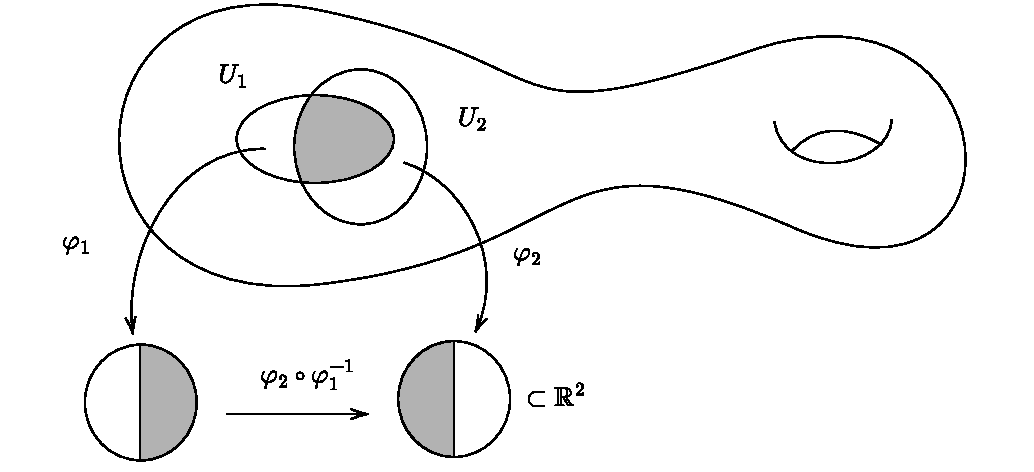
\includegraphics[scale=.7]{Geo1}
\end{center}

Recall from Analysis and Topology that if \( V \subseteq \mathbb R^n \) and \( V' \subseteq \mathbb R^m \) are open, then a continuous map \( f \colon V \to V' \) is called \textbf{smooth} if it is infinitely differentiable.
Equivalently, it is smooth if partial derivatives of all orders in all variables exist at all points.
If \( n = m \), then in particular the homeomorphism \( f \colon V \to V' \) is called a \textbf{diffeomorphism} if it is smooth and has smooth inverse.

\begin{definition}
	An \textbf{abstract smooth surface} is a topological space \( \Sigma \) together with an atlas of charts \( (U_i, \varphi_i) \) such that all transition maps \( \varphi_i \circ \varphi_j^{-1} \colon \varphi_j(U_i \cap U_j) \to \varphi_i(U_i \cap U_j) \) are diffeomorphisms.
\end{definition}

\begin{remark}
	We could not simply consider a smoothness condition for \( \Sigma \) itself without appealing to atlases, since \( \Sigma \) is an arbitrary topological space and could have almost any topology.
\end{remark}

\begin{example}
	The atlas of two charts with stereographic projections gives \( S^2 \) the structure of an abstract smooth surface.
\end{example}

\begin{example}
	The torus \( T^2 = {\mathbb R^2}/{\mathbb Z^2} \). Recall that we obtained charts from (the inverse of) the projection restricted to small discs in $ \mathbb{R}^{2} $. We can find charts of all points by choosing sufficiently small discs in \( \mathbb R^2 \) such that they do not intersect any of their non-trivial integer translates.

	\begin{center}
	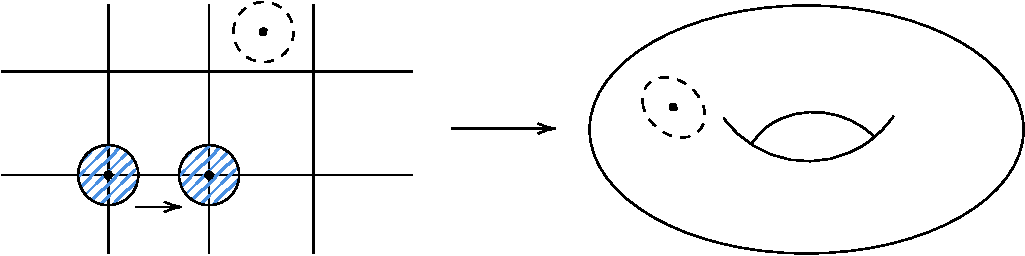
\includegraphics[scale=0.65]{TorusChart1}
	\end{center}

	The transition maps for this atlas are all translations of \( \mathbb R^2 \).
	Hence \( T^2 \) inherits the structure of an abstract smooth surface.
	Explicitly, let us define \( e \colon \mathbb R^2 \to T^2 \) by \( (t,s) \mapsto \qty(e^{2\pi i t}, e^{2 \pi i s}) \), then consider the atlas
	\[
		\qty{(e\qty(D_\varepsilon(x,y)), e^{-1} \text{ on this image})}
	\]
	for \( \varepsilon < \frac{1}{3} \).
	These are charts on \( T^2 \), and the transition maps are (restricted to appropriate domains) translations in \( \mathbb R^2 \).
	Hence \( T^2 \), via this atlas, has the structure of an abstract smooth surface.
\end{example}

\begin{definition}
	Let \( \Sigma \) be an abstract smooth surface, and \( f \colon \Sigma \to \mathbb R^n \) be a continuous map.
	We say that \( f \) is \textbf{smooth} at \( p \in \Sigma \) if, for all charts \( (U, \varphi) \) at \( p \) belonging to the smooth atlas for \( \Sigma \), the map
	\[
		f \circ \varphi^{-1} \colon \mathbb{R}^{2}\supset \varphi(U) \to \mathbb R^n
	\]
	is smooth at \( \varphi(p) \in \mathbb R^2 \).
\end{definition}

\begin{center}
	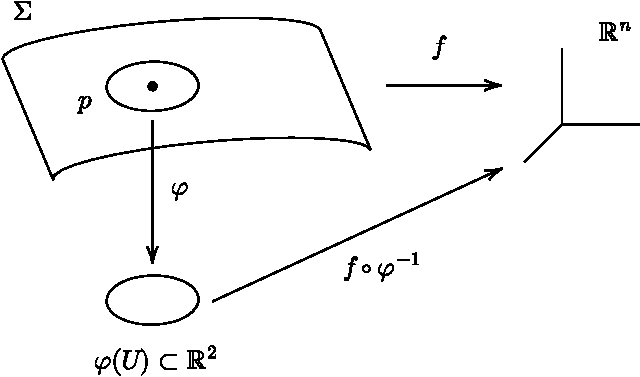
\includegraphics[scale=0.8]{SmoothFunction}
\end{center}

\begin{note}
	If it holds for one chart at $p$, it holds for all charts at $p$ by chain rule: $ f\circ \varphi_1^{-1} = f\circ \varphi_2^{-1} \circ (\varphi_2\circ \varphi_1^{-1}) $, where $ \varphi_2\circ \varphi_1^{-1} $ is a diffeomorphism. 
\end{note}

\begin{definition}
	Let \( \Sigma_1, \Sigma_2 \) be abstract smooth surfaces.
	A map \( f \colon \Sigma_1 \to \Sigma_2 \) is \textbf{smooth} if it is `smooth in the local charts'.
	Given a chart \( (U, \varphi) \) at \( p \) and a chart \( (V, \psi) \) at \( f(p) \) with $ f(U) \subset V $, both mapping to open subsets of \( \mathbb R^2 \), the map \( \psi \circ f \circ \varphi^{-1} \) is smooth at \( \varphi(p) \).
	Smoothness of \( f \) does not depend on the choice of chart, provided that the charts all belong to the same atlas.
\end{definition}
Again is $f$ is smooth at $p$, then smoothness of the local representation of $f$ at $p$ will hold for all charts at $p$ and $f(p)$ in the given atlases, again by chain rule.
\begin{center}
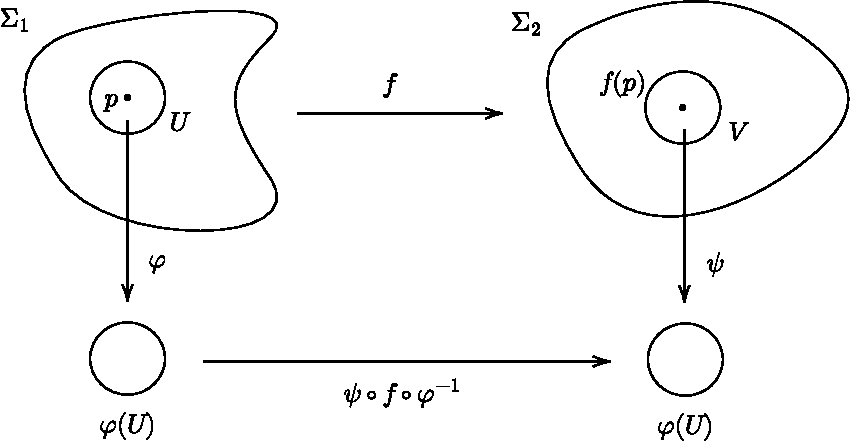
\includegraphics[scale=0.8]{SmoothFunction2}
\end{center}
\begin{definition}
	Two surfaces \( \Sigma_1, \Sigma_2 \) are \textbf{diffeomorphic} if there exists a homeomorphism \( f \colon \Sigma_1 \to \Sigma_2 \) which is smooth and has smooth inverse.
\end{definition}
\begin{remark}
	Often, we convert from a given smooth atlas for an abstract smooth surface \( \Sigma \) to the \textit{maximal compatible} smooth atlas.
	That is, we consider the atlas with the maximal possible set of charts, all of which have transition maps that are diffeomorphisms.
	This can be accomplished formally by use of Zorn's lemma.
\end{remark}

\section{Smooth surfaces in \( \mathbb R^3 \)}
\subsection{Definitions and equivalent characterisations}
Recall that if \( V \subseteq \mathbb R^n \) and \( V' \subseteq \mathbb R^m \), then \( f \colon V \to V' \) is smooth if it is infinitely differentiable.
\begin{definition}
	If \( Z \) is an arbitrary subset of \( \mathbb R^n \), we say that a continuous function \( f \colon Z \to \mathbb R^m \) is smooth at \( p \in Z \) if there exists an open ball \( p \in B \subseteq \mathbb R^n \) and a smooth map \( F \colon B \to \mathbb R^m \) which extends \( f \) such that they agree on \( B \cap Z \).
	In other words, \( f \) is locally the restriction of a smooth map defined on an open set.
\end{definition}
\begin{definition}
	Let \( X \subseteq \mathbb R^n \) and \( Y \subseteq \mathbb R^m \).
	We say that \( X \) and \( Y \) are \textbf{diffeomorphic} if there exists a continuous function \( f \colon X \to Y \) such that \( f \) is a smooth homeomorphism with smooth inverse.
\end{definition}

\begin{definition}
	A \textbf{smooth surface in \( \mathbb R^3 \)} is a subset \(\Sigma \subset \mathbb R^3 \) such that for all points \( p \in \Sigma \), there exists an open subset \( p \in U \subseteq \Sigma \) that is diffeomorphic to an open set in \( \mathbb R^2 \).
	In other words, for all \( p \in \Sigma \), there exists an open ball \( p \in B \subseteq \mathbb R^3 \) such that if \( U = B \cap \Sigma \) and there exists a map \( F \colon B \to V \subseteq \mathbb R^2 \) such that \( {F}\restriction_U \colon U \to V \) is a homeomorphism, and the inverse map \( V \to U \subseteq \Sigma \subseteq \mathbb R^3 \) is smooth.
\end{definition}

\begin{definition}
	Let \( \sigma \colon V \to U \) where \( V \subseteq \mathbb R^2 \) is open and \( U \subseteq \Sigma \subseteq \mathbb R^3 \) is open in \( \Sigma \), such that \( \sigma \) is a smooth homeomorphism and \( D \eval{\sigma}_x \) has rank 2 for all \( x \in V \).
	Then \( \sigma \) is called an \textbf{allowable parametrisation}.
	If \( \sigma(0) = p \), we say that \( \sigma \) is an allowable parametrisation \textbf{near} \( p \).
\end{definition}
\begin{theorem}
	For a subset \( \Sigma \subseteq \mathbb R^3 \), the following are equivalent.
	\begin{enumerate}[(a)]
		\item \( \Sigma \) is a smooth surface in \( \mathbb R^3 \);
		\item \( \Sigma \) is locally the graph of a smooth function, over one of the three coordinate planes: for all \( p \in \Sigma \) there exists an open ball \( p \in B \subseteq \mathbb R^3 \) and an open set \( V \subseteq \mathbb R^2 \) such that
		      \[
			      \Sigma \cap B = \qty{(x, y, g(x,y)) \colon g \colon V \to \mathbb R \text{ smooth}}
		      \]
		      or one of the other coordinate planes;
		\item \( \Sigma \) is locally cut out by a smooth function with non-zero derivative: for all \( p \in \Sigma \) there exists an open ball \( p \in B \subseteq \mathbb R^3 \) and a smooth function \( f \colon B \to \mathbb R \) such that
		      \[
			      \Sigma \cap B = f^{-1}(0);\quad D \teval{f}{x} \neq 0
		      \]
		      for all \( x \in B \);
		\item \( \Sigma \) is locally the image of an allowable parametrisation near all points.
	\end{enumerate}
\end{theorem}
\begin{remark}
	Part (b) implies that if \( \Sigma \) is a smooth surface in \( \mathbb R^3 \), each \( p \in \Sigma \) belongs to a chart \( (U, \varphi) \) where \( \varphi \) is (the restriction of) one of the three coordinate plane projections \( \pi_{xy}, \pi_{yz}, \pi_{xz} \) from \( \mathbb R^3 \) to \( \mathbb R^2 \).
	Consider the transition map between two such charts.
	If the two charts are based on the same projection such as \( \pi_{xy} \), then the transition map is the identity.
	If they are based on different projections \( \pi_{xy} \) and \( \pi_{yz} \), then the transition map is
	\[
		(x,y) \mapsto (x,y,g(x,y)) \mapsto (y,g(x,y))
	\]
	which has inverse
	\[
		(y,z) \mapsto (h(y,z),y,z) \mapsto (h(y,z),y)
	\]
	Hence all of the transition maps between such charts involve projection maps and the smooth maps involved in defining \( \Sigma \) as a graph.
	This gives \( \Sigma \) the structure of an abstract smooth surface.
\end{remark}
Some of the relations given in the above theorem are easy to prove, but others come as a result of the inverse function theorem.

\subsection{Inverse and implicit function theorems}
\ \vspace*{-1.5em}

\begin{theorem}[Inverse function theorem]
	Let \( U \subseteq \mathbb R^n \) be open, and \( f \colon U \to \mathbb R^n \) be continuously differentiable.
	Let \( p \in U \) and \( f(p) = q \).
	Suppose \( \eval{Df}_p \) is invertible.
	Then there is an open neighbourhood \( V \) of \( q \) and a differentiable map \( g \colon V \to \mathbb R^n \) and \( g(q) = p \) with image an open neighbourhood \( U' \subseteq U \) of \( p \) such that \( f \circ g = \id_V \) and $ g\circ f = \id_{U'} $.
	If \( f \) is smooth, so is $g$.
\end{theorem}
\begin{remark}
	The chain rule then implies that \( \eval{Dg}_q = \qty(\eval{Df}_p)^{-1} \).
\end{remark}

The inverse function theorem concerns functions \( \mathbb R^n \to \mathbb R^n \), where \( \eval{Df}_p \) is an isomorphism.
If we have a map \( \mathbb R^n \to \mathbb R^m \) for \( n > m \), then we can discuss the behaviour when \( \eval{Df}_p \) is surjective.
The derivative \( \eval{Df}_p \) is an \( n \times m \) matrix:
\[
	{\textstyle\eval{Df}_p} = \left( \pdv{f_i}{x_j} \right)_{m\times n},
\]
so if it has full rank, up to the permutation of coordinates we have that the first or last \( m \) columns are linearly independent.

\begin{theorem}[Implicit function theorem]
	Let \( p = (x_0, y_0) \) be a point in an open set \( U \subset \mathbb R^k \times \mathbb R^\ell \).
	Let \( f \colon U \to \mathbb R^\ell \) be a continuously differentiable map such that \( p \mapsto 0 \) and \( \qty(\pdv{f_i}{y_j})_{\ell \times \ell} \) is an isomorphism.
	Then there is an open neighbourhood \( V \) of \( x_0 \) in \( \mathbb R^k \) and a continuously differentiable map \( g \colon V \to \mathbb R^\ell \) with \( x_0 \mapsto y_0 \) such that if \( (x,y) \in U \cap (V \times \mathbb R^\ell) \), then \( f(x,y)=0\iff y=g(x) \).
	If \( f \) is smooth, so is \( g \).
\end{theorem}
\begin{proof}
	Introduce $ F:U\to \mathbb{R}^{k} \times \mathbb{R}^{\ell} $ such that $ (x,y) \mapsto (x,f(x,y)) $. Then 
	\[
		DF = \begin{pmatrix}
			I & \ast           \\
			0 & \pdv{f_i}{y_j}
		\end{pmatrix}
	\]
	hence \( DF \) is an isomorphism at \( (x_0, y_0) \) by assumption. By the inverse function theorem, \( F \) is locally invertible near \( F(x_0,y_0) = (x_0,f(x_0,y_0)) = (x_0, 0) \).

	 Take a product open neighbourhood \( V \times V' \subseteq \mathbb R^k \times \mathbb R^\ell \) on which this continuously differentiable inverse \( G \colon V \times V' \to U' \subseteq U \subseteq \mathbb R^k \times \mathbb R^\ell \) exists, such that \( F \circ G = \id_{V \times V'} \).
	 Then,
	\[
		G(x,y) = (\varphi(x,y), \psi(x,y)) \implies F \circ G(x,y) = (\varphi(x,y), f(\varphi(x,y), \psi(x,y))) = (x,y)
	\]
	This implies \( \varphi(x,y) = x \).
	We have \( f(x,\psi(x,y)) = y \) when \( (x,y) \in V \times V' \).
	This gives \( f(x,y) = 0 \iff y = \psi(x,0) \).
	We then define \( g \colon V \to \mathbb R^\ell \) by \( x \mapsto \psi(x,0) \).
\end{proof}

\begin{example}
	Let \( f \colon \mathbb R^2 \to \mathbb R \) be smooth and \( f(x_0, y_0) = 0 \), and suppose \( \pdv{f}{y} \neq 0 \) at \( (x_0, y_0) \).
	Then there exists a smooth map \( g \colon (x_0 - \varepsilon, x_0 + \varepsilon) \to \mathbb R \) with \( g(x_0) = y_0 \) and \( f(x,y) = 0 \iff y = g(x) \) for \( (x,y) \) in some open neighbourhood of \( (x_0, y_0) \).
	Since \( f(x,g(x)) = 0 \) in this open neighbourhood, we can differentiate that expression to find
	\[
		g'(x) = \frac{-f_x}{f_y}
	\]
	noting that \( f_y \neq 0 \) in some neighbourhood near \( (x_0, y_0) \).
	Note that the level set \( f(x,y) = 0 \) is implicitly defined by \( g \), which is a function for which we have an integral expression.
	\begin{center}
		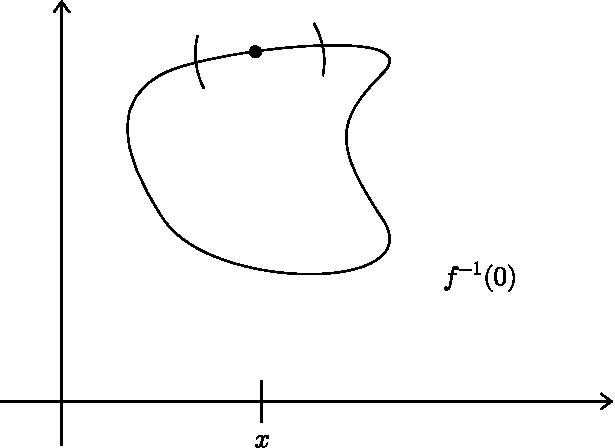
\includegraphics[scale=0.8]{Implicit}
	\end{center}
\end{example}

\begin{example}
	Let \( f \colon \mathbb R^3 \to \mathbb R \) be a smooth map with \( f(x_0, y_0, z_0) = 0 \).
	Consider the level set \( \Sigma = f^{-1}(0) \), assuming that \( Df \neq 0 \) at \( (x_0, y_0, z_0) \).
	Permuting coordinates if necessary, we can assume \( \pdv{f}{z} \neq 0 \) at this point.
	Then there exists an open neighbourhood \( V \) of \( (x_0, y_0) \) and a smooth function \( g \colon V \to \mathbb R \) such that \( (x_0, y_0) \mapsto z_0 \) with the property that for an open set \( (x_0, y_0, z_0) \in U \), the set \( f^{-1}(0) \cap U = \Sigma \cap U \) is the graph of the function \( g \), which is \( \qty{ (x,y,g(x,y)) \colon (x,y) \in V } \).
\end{example}

We now prove the theorem stated above, relating equivalent conditions for smoothness of a surface \( \Sigma \).
\begin{proof}
	First, we show that (b) implies all of the other conditions.
	If \( \Sigma \) is locally a graph \( \qty{(x,y,g(x,y))} \), we find a chart from the coordinate plane projection \( \pi_{xy} \) of that graph.
	Since this projection is smooth and defined on an open neighbourhood of points of \( \Sigma \) in its domains, this shows that \( \Sigma \) is a smooth surface in \( \mathbb R^3 \) (a).
	Further, since \( \Sigma \) is locally the given graph, it is cut out by the function \( f(x,y,z) = z - g(x,y) \) and \( \pdv{f}{z} \neq 0 \) (c).
	Finally, the local parametrisation \( \sigma(x,y) = (x,y,g(x,y)) \) is allowable; \( g \) is smooth, the partial derivatives of \( \sigma \) are linearly independent by considering the \( x \) and \( y \) components, and \( \sigma \) is injective where required (d).

	Now, we show (a) implies (d).
	This is simply part of the definition of being a smooth surface in \( \mathbb R^3 \), being locally diffeomorphic to \( \mathbb R^2 \).
	In particular, at \( p \in \Sigma \), \( \Sigma \) is locally diffeomorphic to \( \mathbb R^2 \) and the inverse of such a local diffeomorphism is an allowable parametrisation.

	We have already shown (c) implies (b); this was the example of the implicit function theorem provided above.

	Finally, we must prove (d) implies (a) and (b), and then the result will hold.
	Let \( p \in \Sigma \) and \( V \) be an open set in \( \mathbb R^2 \) with an allowable parametrisation to \( \Sigma \) such that \( \sigma(0) = p \).
	If \( \sigma = (\sigma_1(u,v), \sigma_2(u,v), \sigma_3(u,v)) \), we have
	\[
		D\sigma = \begin{pmatrix}
			\pdv{\sigma_1}{u} & \pdv{\sigma_1}{v} \\[.5em]
			\pdv{\sigma_2}{u} & \pdv{\sigma_2}{v} \\[.5em]
			\pdv{\sigma_3}{u} & \pdv{\sigma_3}{v}
		\end{pmatrix}
	\]
	This has rank 2, hence there exist two rows defining an invertible matrix.
	Suppose those are the first two rows, and let \( \mathrm{pr} = \pi_{xy} \) be the projection map.
	Consider \( \mathrm{pr} \circ \sigma \colon V \to \mathbb R^2 \).
	This has isomorphic derivative at zero, so we can apply the inverse function theorem.
	Hence \( \Sigma \) is locally a graph over the \( xy \) coordinate plane, so (b) holds.
	Moreover, let \( \varphi = \mathrm{pr} \circ \sigma \), and consider the open ball \( B(p, \delta) \subseteq \mathbb R^3 \) and a map such that \( (x,y,z) \mapsto \varphi^{-1}(x,y) \) in this ball.
	Here, \( \varphi \colon W \to \Sigma \) where \( W \) is an open set in \( \mathrm{pr}(B(p, \delta)) \).
	This is a locally defined map, which is smooth on an open set in \( \mathbb R^3 \), which is a smooth inverse to \( \sigma \).
	Hence \( \Sigma \) is a smooth surface in \( \mathbb R^3 \), so (a) holds.
\end{proof}

\begin{example}
	The ellipsoid \( f^{-1}(0) \) for \( f(x,y,z) = x^2/a^2 + y^2/b^2 + z^2/c^2 - 1 \).
	For any point, \( Df \neq 0 \), so it is a smooth surface.
\end{example}
\begin{example}
	Let \( \gamma \colon [a,b] \to \mathbb R^3 \) be a smooth map with image in the \( xz \) plane, so
	\[
		\gamma(t) = (f(t), 0, g(t))
	\]
	such that \( \gamma \) is injective, \( \gamma' \neq 0 \), and \( f > 0 \).
	The \textbf{surface of revolution} of \( \gamma \) has allowable parametrisation
	\[
		\sigma(u,v) = (f(u)\cos v, f(u)\sin v, g(u))
	\]
	where \( (u,v) \in (a,b) \times (\theta, \theta + 2\pi) \) for a fixed \( \theta \).
	\begin{center}
	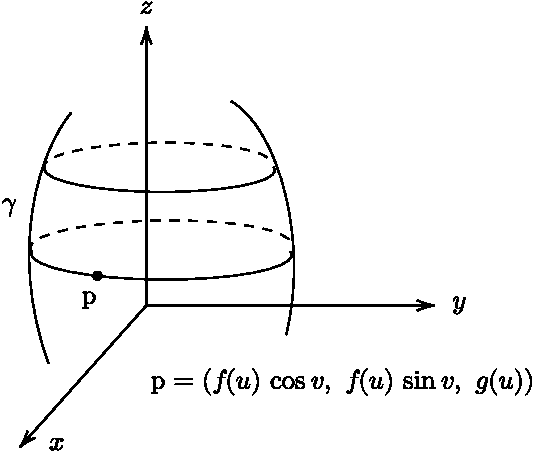
\includegraphics[scale=0.8]{SoR}
	\end{center}
	Note that \( \sigma_u = (f_u \cos v, f_u \sin v, g_u) \) and \( \sigma_v = (-f\sin v, f \cos v, 0) \), and we can check \( \norm{\sigma_u \times \sigma_v} = f^2 ((f')^2 + (g')^2) \) which is nonzero on \( \gamma \), so this really is an allowable parametrisation.
\end{example}

\subsection{Orientability}
Let \( V, V' \) be open sets in \( \mathbb R^2 \).
	Let \( f \colon V \to V' \) be a diffeomorphism.
	Then at every point \( x \in V \), \( \eval{Df}_x \in \GL(2,\mathbb R) \); it is invertible since \( f \) is a diffeomorphism.
	Let \( \GL^+(2,\mathbb R) \) be the subgroup of matrices with positive determinant.
\begin{definition}
	We say that \( f \) is \textbf{orientation-preserving} if $ Df|_x\in \GL^+(2,\mathbb R) $ for all points \( x \in V \).
\end{definition}
\begin{definition}
	An abstract smooth surface \( \Sigma \) is \textbf{orientable} if it admits an atlas \( \qty{(U_i, \varphi_i)} \) where the transition maps are all orientation-preserving.
	A choice of such an atlas is an \textbf{orientation} of \( \Sigma \); \( \Sigma \) can be called \textbf{oriented} when such an orientation is given.
\end{definition}
\begin{remark}
	An orientable atlas belongs to a maximal compatible oriented smooth atlas.
\end{remark}
\begin{lemma}
	If \( \Sigma_1 \) and \( \Sigma_2 \) are diffeomorphic abstract smooth surfaces, then \( \Sigma_1 \) is orientable if and only if \( \Sigma_2 \) is orientable.
\end{lemma}
\begin{proof}
	Let \( f \colon \Sigma_1 \to \Sigma_2 \) be a diffeomorphism.
	Suppose \( \Sigma_2 \) is orientable and equipped with an oriented smooth atlas.
	Consider the atlas on \( \Sigma_1 \) of charts of the form \( (f^{-1}(U), \eval{\phi \circ f}_{f^{-1}(U)}) \), where \( (U, \psi) \) is a chart at \( f(p) \) in the oriented atlas for \( \Sigma_2 \).
	Then, the transition map between two such charts is exactly a transition map between charts in the \( \Sigma_2 \) atlas.
	\begin{center}
		\begin{tikzcd}
			f^{-1}(U)\in \Sigma_1 \arrow[r, "f"] \arrow[rd, "\varphi\circ f"'] & U\in \Sigma_2 \arrow[d, "\varphi"] \\
			& \varphi(U)\in \mathbb{R}^2        
		\end{tikzcd}
	\end{center}
	In other words, in the maximal smooth atlas that exists a priori for \( \Sigma_1 \), we will allow charts of the form \( (\widetilde U, \widetilde \psi) \) when for all charts \( (U, \psi) \) at \( f(p) \) in the \( \Sigma_2 \) atlas, the map \( \psi \circ f \circ (\widetilde \psi)^{-1} \) is orientation-preserving.
	Informally, if the atlas on \( \Sigma_2 \) was maximal as an oriented atlas, we can recover the previous set of charts.
\end{proof}

\begin{remark}
	(1) There is no sensible classification of the set of all smooth surfaces.
	For instance, \( \mathbb R^2 \setminus Z \) for a closed set \( Z \) can be shown to yield uncountably many types of homeomorphisms.
	However, \textit{compact} smooth surfaces may be classified by their Euler characteristic and their orientability, up to diffeomorphism.
	This theorem will not be proven in this course.

	(2) There is a definition of orientation-preserving \textit{homeomorphism} that does not rely on the determinant, but that instead relies on some algebraic topology which is not covered in this course.
	The M\"obius band is the surface
	\begin{center}
		\begin{tikzpicture}
				\node (0) at (-2, 1) {};
				\node (1) at (-2, -1) {};
				\node (2) at (2, -1) {};
				\node (3) at (2, 1) {};
				\node (4) at (-2, 0) {};
				\node (5) at (2, 0) {};
				\draw [->] (1.center) to (4.center);
				\draw [->] (3.center) to (5.center);
				\draw (5.center) to (2.center);
				\draw (4.center) to (0.center);
				\draw [dashed] (0.center) to (3.center);
				\draw [dashed] (2.center) to (1.center);
		\end{tikzpicture}
	\end{center}
	where the dashed lines represent the absence of edges.
	It turns out that an abstract smooth surface is orientable if and only if it contains no subsurface homeomorphic to the M\"obius band.
	We can therefore say that a topological surface is orientable if and only if it contains no subsurface (an open set) homeomorphic to a M\"obius band.

	(3) We can define other structures on an abstract smooth surface by considering smooth atlases such that if \( \varphi_1 \varphi_2^{-1} \) is a transition map, then \( D (\varphi_1 \varphi_2^{-1}) \) at \( x \) belongs to a specific subgroup \( G \leq \GL(2, \mathbb R) \).
	For example, defining \( G = \qty{e} \) leads to Euclidean surfaces.
	The group \( \GL(1, \mathbb C) \) identified as a subgroup of \( \GL(2, \mathbb R) \) yields the Riemann surfaces.
\end{remark}

\begin{example}
	For \( S^2 \) with the atlas of two stereographic projections, we can find the transition map to be
	\[
		(u,v) \mapsto \qty(\frac{u}{u^2 + v^2}, \frac{v}{u^2 + v^2})
	\]
	on \( \mathbb R^2 \setminus \qty{0} \).
	This has positive determinant, so \( S^2 \) is orientable.

	For the torus \( T^2 \), we previously found an atlas such that the transition maps are translations of \( \mathbb R^2 \).
	Hence the torus is an oriented surface, and also a Euclidean surface.
\end{example}

\subsection{Tangent planes}
An \textbf{affine} subspace of a vector space is a translate of a linear subspace.
\begin{definition}
	Let \( \Sigma \) be a smooth surface in \( \mathbb R^3 \), and \( p \in \Sigma \).
	Let \( \sigma \colon V \to U \subseteq \Sigma \) be an allowable parametrisation of \( \Sigma \) near \( p \), so \( V \) is an open subset of \( \mathbb R^2 \) and \( U \) is open in \( \Sigma \), such that \( \sigma(0) = p \).
	The \textbf{tangent plane} \( T_p \Sigma \) to \( p \) at \( \Sigma \) is the image of \( \qty(D \eval{\sigma}_0) \subseteq \mathbb R^3 \), which is a two-dimensional vector subspace of \( \mathbb R^3 \).
	The \textbf{affine tangent plane} is \( p + T_p \Sigma \), which is an affine subspace of \( \mathbb R^3 \).
\end{definition}
\begin{lemma}
	\( T_p \Sigma \) is independent of the choice of allowable parametrisation.
\end{lemma}

\begin{proof}[Proof (i)]
	Suppose \( \sigma \colon V \to U \) and \( \widetilde \sigma \colon \widetilde V \to \widetilde U \) are allowable parametrisations with \( \sigma(0) = \widetilde \sigma(0) = p \).
	There exists a transition map \( \sigma^{-1} \circ \widetilde \sigma \), which is a diffeomorphism of open sets in \( \mathbb R^2 \).
	Therefore,
	\[
		\widetilde \sigma = \sigma \circ \underbrace{\qty(\sigma^{-1} \circ \widetilde \sigma)}_{\text{diffeomorphism}}
	\]
	Hence \( D\eval{(\sigma^{-1} \circ \widetilde \sigma)}_{0} \) is an isomorphism.
	Thus, the images of \( D \eval{\widetilde \sigma}_0 \) and \( D \eval{\sigma}_0 \) agree.
\end{proof}
\begin{proof}[Proof (ii)]
	Let \( \gamma \colon (-\varepsilon, \varepsilon) \to \mathbb R^3 \) be a smooth map such that \( \gamma \) has image inside \( \Sigma \), and \( \gamma(0) = p \).
	We will show that \( \gamma'(0) \in T_p \Sigma \).
	If \( \sigma \colon V \to U \) is an allowable parametrisation with \( \sigma(0) = p \) as above, and \( \varepsilon \) is sufficiently small such that \( \Im \gamma \subseteq U \), then \( \gamma(t) = \sigma(u(t), v(t)) \) for some smooth functions \( u, v \colon (-\varepsilon, \varepsilon) \to V \).
	Then \( \gamma'(t) = \sigma_u u'(t) + \sigma_v v'(t) \) is in the image of \( D \eval{\sigma}_t \).
	Thus, \( T_p \Sigma = \spn \qty{ \gamma'(0) \colon \gamma \text{ as above} } \).
\end{proof}

\begin{definition}
	If \( \Sigma \) is a smooth surface in \( \mathbb R^3 \) and \( p \in \Sigma \), the \textbf{normal direction} to \( \Sigma \) at \( p \) is \( (T_p \Sigma)^\perp \), the Euclidean orthogonal complement to the tangent plane at \( p \).
\end{definition}
\begin{remark}
	For all \( p \in \Sigma \), there exist exactly two normalised normal vectors.
\end{remark}
\begin{definition}
	A smooth surface in \( \mathbb R^3 \) is \textbf{two-sided} if it admits a continuous global choice of unit normal vector.
\end{definition}
\begin{lemma}
	A smooth surface in \( \mathbb R^3 \) is orientable (as an abstract smooth surface) if and only if it is two-sided (as a smooth surface in \( \mathbb R^3 \)).
\end{lemma}

\begin{proof}
	Let \( \sigma \colon V \to U \subseteq \Sigma \) be an allowable parametrisation.
	Let \( \sigma(0) = p \).
	We will define the positive unit normal with respect to \( \sigma \) at \( p \) to be the normal vector \( n_\sigma(p) \) with the property that \( \qty{\sigma_u, \sigma_v, n_\sigma(p)} \) and \( \qty{e_1, e_2, e_3} \) are related by a positive determinant change of basis matrix, where \( \qty{e_1, e_2, e_3} \) are the standard basis vectors.
	\begin{center}
		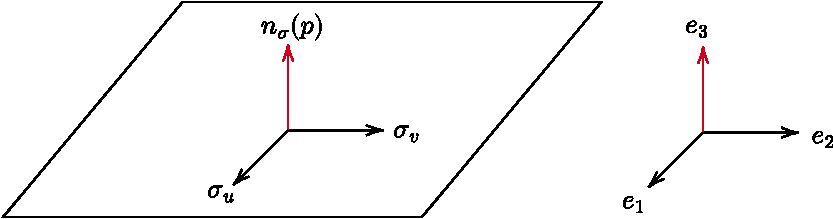
\includegraphics[scale=.8]{orientable-lemma}
	\end{center}
	In other words,
	\[
		n_\sigma(p) = \frac{\sigma_u \times \sigma_v}{\norm{\sigma_u \times \sigma_v}}
	\]
	Consider an alternative parametrisation \( \widetilde \sigma \colon \widetilde V \to \widetilde U \), where \( \widetilde \sigma(0) = p \), such that \( \widetilde \sigma \) belongs to the same oriented and smooth atlas as \( \sigma \).
	Hence, \( \sigma = \widetilde \sigma \circ \varphi \) for some transition map \( \varphi \).
	Let
	\[
		{\textstyle \eval{D \varphi}_0} = \begin{pmatrix}
			\alpha & \beta  \\
			\gamma & \delta
		\end{pmatrix}
	\]
	Hence,
	\[
		\sigma_u = \alpha \widetilde \sigma_u + \gamma \widetilde \sigma_v;\quad \sigma_v = \beta \widetilde \sigma_u + \delta \widetilde \sigma_v
	\]
	This gives
	\begin{equation}
		\sigma_u \times \sigma_v = \det\qty({\textstyle \eval{D  \varphi}_0}) \widetilde \sigma_u \times \widetilde \sigma_v \tag{\(\dagger\)}
	\end{equation}
	The determinant here is positive since the charts in question belong to an oriented atlas.
	Thus, the positive normal depends on the orientation of \( \Sigma \), but does not depend on the choice of parametrisation.
	The expression for \( n_\sigma(p) \) is continuous since the cross product is continuous, hence \( \Sigma \) is two-sided.

	Conversely, if \( \Sigma \) is two-sided and there exists a global continuous choice of normal vector, we can consider the subatlas of the natural smooth atlas with the property that we allow \( (U,\varphi) \) if the associated parametrisation \( \sigma = \varphi^{-1} \) satisfies \( \qty{\sigma_u, \sigma_v, n} \) is a positive basis for \( \mathbb R^3 \), where \( n \) is the given choice of normal.
	By (\(\dagger\)), the transition maps between such charts are orientation-preserving.
	Hence \( \Sigma \) is orientable.
\end{proof}

\begin{lemma}
	If \( \Sigma \) is a smooth surface in \( \mathbb R^3 \) and \( A \colon \mathbb R^3 \to \mathbb R^3 \) is a smooth map which preserves \( \Sigma \) setwise, then \( \eval{DA}_p \in L(\mathbb R^3, \mathbb R^3) \) maps \( T_p \Sigma \) to \( T_{A(p)} \Sigma \) for \( p \in \Sigma \).
\end{lemma}
\begin{proof}
	Let \( \gamma \colon (-\varepsilon, \varepsilon) \to \mathbb R^3 \) be a smooth map such that its image lies on \( \Sigma \), and \( \gamma(0) = p \).
	Recall that \( T_p \Sigma \) is spanned by \( \gamma'(0) \) for such curves \( \gamma \).
	Now, consider \( A \circ \gamma \colon (-\varepsilon, \varepsilon) \to \mathbb R^3 \), which also has image \( \Sigma \), and
	\[
		\teval{DA}{\gamma(0)} \circ \teval{D\gamma}{0} = \teval{DA}{p} \qty(\gamma'(0)) = \teval{D(A \circ \gamma)}{0} \in T_{A(p)} \Sigma
	\]
\end{proof}
\begin{example}
	Let \( S^2 \) be the unit sphere.
	The normal vector at \( p \) is the line through the origin and \( p \); indeed, since \( \SO_3 \) acts transitively on \( S^2 \), it suffices to check at one point, such as the north pole. Take any $ \gamma:(-\epsilon,\epsilon)\to S^2, \gamma(0)=p, $ then $ \left\| \gamma(t) \right\|^2 = 1 $. Differentiating on both sides gives $ \inner{\gamma'(0),p} = 0 $, i.e. $ (T_p S^2)^{\perp} = \mathbb{R} p $. 

	We can choose the outward-facing normal vector to be the positive normal, denoted \( n(p) \).
	\( S^2 \) is two-sided by the construction of this normal vector, hence \( S^2 \) is orientable.
\end{example}

\begin{example}
	One embedding of the M\"obius band in \( \mathbb R^3 \) is
	\[
		\sigma(t,\theta) = \qty(\qty(1 - t \sin \frac{\theta}{2})\cos \theta, \qty(1 - t \sin \frac{\theta}{2})\sin \theta, t \cos \frac{\theta}{2})
	\]
	where \( (t,\theta) \in V_1 = \qty{t \in \qty(-\frac{1}{2}, \frac{1}{2}), \theta \in (0,2\pi)} \) or \( (t,\theta) \in V_2 = \qty{t \in \qty(-\frac{1}{2}, \frac{1}{2}), \theta \in (-\pi, \pi)} \).
	We begin with the unit circle \( x^2 + y^2 = 1 \), for \( t = 0 \).
	Then, at each point on the circle, we consider an open interval of unit length, which will rotate as we move around the circle, such that at the point \( \theta \) on the circle it has rotated by \( \frac{\theta}{2} \).
	We can check that if \( \sigma_i \) is \( \sigma \) on \( V_i \), then \( \sigma_i \) is allowable.
	Further,
	\[
		\sigma_t \times \sigma_\theta = \qty(-\cos\theta \cos\frac{\theta}{2}, -\sin\theta \cos\frac{\theta}{2}, -\sin\frac{\theta}{2}) =: n_\theta
	\]
	which is already normalised.
	As \( \theta \to 0 \) from above, \( n_\theta \to (-1,0,0) \).
	As \( \theta \to 2\pi \) from below, \( n_\theta \to (1,0,0) \).
	Hence, the surface is not two-sided and not orientable. 
\end{example}

\section{Geometry of surfaces in \( \mathbb R^3 \)}
\subsection{First fundamental form}

Let \( \gamma \colon (a,b) \to \mathbb R^3 \) be smooth.
The \textbf{length} of \( \gamma \) is
\[
	L(\gamma) = \int_a^b \norm{\gamma'(t)} \dd{t}
\]
This result is independent of the choice of parametrisation.
Let \( s \colon (A,B) \to (a,b) \) be a monotonically increasing function, and let \( \tau(t) = \gamma(s(t)) \).
Then
\[
	L(\tau) = \int_A^B \norm{\tau'(t)} \dd{t} = \int_A^B \norm{\gamma'(s(t))} \abs{s'(t)} \dd{t} = \int_a^b \norm{\gamma'(t')} \dd{t'} = L(\gamma)
\]
By using inverse function theorem, one can show that
\begin{lemma}
	If \( \gamma \colon (a,b) \to \mathbb R^3 \) is continuously differentiable and \( \gamma'(t) \neq 0 \), then \( \gamma \) can be parametrised by arc length.
\end{lemma} 


Let \( \Sigma \) be a smooth surface in \( \mathbb R^3 \), and let \( \sigma \colon V \to U \subseteq \Sigma \) be an allowable parametrisation.
If \( \gamma \colon (a,b) \to \mathbb R^3 \) is smooth and its image is contained within \( U \), then there exist functions \( (u(t), v(t)) \colon (a,b) \to V \) such that \( \gamma(t) = \sigma(u(t), v(t)) \).
Hence \( \gamma'(t) = \sigma_u u'(t) + \sigma_v v'(t) \), giving
\[
	\norm{\gamma'(t)}^2 = E u'(t)^2 + 2F u'(t) v'(t) + G v'(t)^2
\]
for functions
\[
	E = \inner{\sigma_u, \sigma_u};\quad F = \inner{\sigma_u, \sigma_v} = \inner{\sigma_v, \sigma_u};\quad G = \inner{\sigma_v, \sigma_v}
\]
where \( \inner{\cdot,\cdot} \) represents the usual Euclidean inner product.
Note that \( E, F, G \) depend only on \( \sigma \) and not on \( \gamma \).
\begin{definition}
	The \textbf{first fundamental form} of \( \Sigma \) in the parametrisation \( \sigma \) is the expression
	\[
		E \dd{u}^2 + 2F \dd{u} \dd{v} + G \dd{v}^2
	\]
	This notation is illustrative of the fact that if \( \gamma \) has image in the image of \( \sigma(v) \), we find
	\[
		L(\gamma) = \int_a^b \sqrt{E (u')^2 + 2F u'v' + G (v')^2} \dd{t}
	\]
	where \( \gamma(t) = \sigma(u(t),v(t)) \).
\end{definition}
\begin{remark}
	The Euclidean inner product on \( \mathbb R^3 \) provides an inner product on the subspace \( T_p \Sigma \).
	Choosing a parametrisation \( \sigma \), we can say \( T_p \Sigma = \Im D \eval{\sigma}_0 = \spn{\qty{\sigma_u, \sigma_v}} \) where \( \sigma(0) = p \).
	The first fundamental form is a quadratic form on the tangent spaces \( T_p \Sigma \), varying smoothly in \( p \).
	However, we choose to express this in a basis coming from the parametrisation \( \sigma \): Let $ I_p(w) = \norm{w}^2 = \inner{w,w}_{\mathbb{R}^3}, w\in T_p\Sigma $, after picking $ \sigma, \sigma(0) = p, w = \eval{D\sigma}_0(u',v' ), $ we have $ I_p(w) = E u'^2 + 2F u'v' + G v'^2 $. 

	In particular, we can think about the matrix expression
	\[
		\begin{pmatrix}
			E & F \\
			F & G
		\end{pmatrix}
	\]
	This is an example of a \textbf{Riemannian metric}. 
\end{remark}

\begin{example}
	The plane \( \mathbb R^2_{xy} \subset \mathbb R^3 \) has the parametrisation \( (u,v) \mapsto (u,v,0) \).
	Hence, \( \sigma_u = e_1 \) and \( \sigma_v = e_2 \), hence the first fundamental form is \( \dd{u}^2 + \dd{v}^2 \).
	We could also use polar coordinates, using \( \sigma(r,\theta) = (r\cos\theta,r\sin\theta,0) \).
	This parametrises the plane without the origin.
	This gives \( \sigma_r = (\cos\theta,\sin\theta,0) \) and \( \sigma_\theta = (-r\sin\theta, r\cos\theta,0) \).
	The first fundamental form is \( \dd{r}^2 + r^2 \dd{\theta}^2 \).
\end{example}
\begin{definition}
	Let \( \Sigma, \Sigma' \) be smooth surfaces in \( \mathbb R^3 \).
	We say that they are \textbf{isometric} if there exists a diffeomorphism \( f\colon \Sigma \to \Sigma' \) that preserves the lengths of all curves.
	More formally, for every smooth curve \( \gamma \colon (a,b) \to \Sigma \), the length of \( \gamma \) is the same as the length of \( f \circ \gamma \).
\end{definition}
\begin{example}
	Let \( \Sigma' = f(\Sigma) \) where \( f \colon \mathbb R^3 \to \mathbb R^3 \) is a global isometry, or rigid motion, of \( \mathbb R^3 \); that is, \( v \mapsto Av+b \) for an orthogonal matrix \( A \).
	These isometries preserve the Euclidean inner product on \( \mathbb R^3 \), hence \( f \) preserves length.
	However, in the definition, we need not map all of \( \mathbb R^3 \) to itself, just \( \Sigma \to \Sigma' \).
\end{example}

\begin{definition}
	We say that \( \Sigma \) and \( \Sigma' \) are \textbf{locally isometric} near points \( p \in \Sigma \) and \( q \in \Sigma' \) if there exist open neighbourhoods \( U \) of \( p \) and \( V \) of \( q \) such that \( U \) and \( V \) are isometric.
	We can also say that \( \Sigma \) and \( \Sigma' \) are locally isometric if they are locally isometric at all points; that is, each point of \( \Sigma \) is locally isometric to some point on \( \Sigma' \).
\end{definition}
\begin{lemma}
	Smooth surfaces \( \Sigma, \Sigma' \) in \( \mathbb R^3 \) are locally isometric near \( p \in \Sigma \) and \( q \in \Sigma' \) if and only if there exist allowable parametrisations \( \sigma \colon V \to U \subseteq \Sigma \) and \( \sigma' \colon V \to U' \subseteq \Sigma' \) such that the first fundamental forms are equivalent.
\end{lemma}
\begin{proof}
	($ \Longleftarrow $) The first fundamental form of \( \Sigma \) determines the lengths of all curves on \( \Sigma \) that lie in \( U \): If we have $ \sigma,\sigma' $ as in the lemma, then $ \sigma'\circ \sigma^{-1} $ is an isometry since 
	\begin{align*}
		\abs{\dv{}{t}\sigma'\circ \sigma^{-1}\circ \gamma(t)}^2 &= \abs{\dv{}{t}\sigma'(u(t),v(t))}\\ 
		&= E'\dot{u}^2+2F' \dot{u}\dot{v}+G'\dot{v}^2\\ 
		&= E\dot{u}^2+2F \dot{u}\dot{v}+G\dot{v}^2 = \abs{\dv{}{t}\gamma(t)}^2
	\end{align*}
	which implies $ L(\sigma'\circ \sigma^{-1}\circ \gamma) = L(\gamma) $. 

	($\Longrightarrow$) We will now show that lengths of curves determine the first fundamental form of a parametrisation.
	Given \( \sigma \colon V \to U \), without loss of generality let \( V = B(0,\delta) \) for some \( \delta > 0 \), where \( \sigma(0) = p \).
	Consider, for all \( \varepsilon < \delta \), the curve
	\[
		\gamma_\varepsilon \colon [0,\varepsilon] \to U;\quad t \mapsto \sigma(t,0)
	\]
	Then,
	\[
		\dv{\varepsilon} L(\gamma_\varepsilon) = \dv{\varepsilon} \int_0^\varepsilon \sqrt{E(t,0)} \dd{t} = \sqrt{E(\varepsilon,0)}
	\]
	Hence,
	\[
		\eval{\dv{\varepsilon}}_{\varepsilon = 0} L(\gamma_\varepsilon) = \sqrt{E(0,0)}
	\]
	So we can determine \( E \) at \( p \) by looking at lengths of curves.
	We can similarly consider
	\[
		\chi_\varepsilon \colon [0,\varepsilon] \to U;\quad t \mapsto \sigma(0,t)
	\]
	which determines \( G \).
	Finally, consider
	\[
		\lambda_\varepsilon \colon [0,\varepsilon] \to U;\quad t \mapsto \sigma(t,t)
	\]
	which determines \( \sqrt{(E+2F+G)(0,0)} \) which gives \( F \) implicitly.
\end{proof}

\begin{example}
	The sphere of radius \( a \), given by \( \qty{x^2 + y^2 + z^2 = a^2} \), has an open set with allowable parametrisation
	\[
		\sigma(u,v) = (a\cos u \cos v, a \cos u \sin v, a \sin u)
	\]
	where \( u \in \qty(-\frac{\pi}{2}, \frac{\pi}{2}) \) and \( v \in (0,2\pi) \).
	This parametrises the complement of a half great circle.
	Here,
	\[
		\sigma_u = (-a \sin u \cos v, -a \sin u \sin v, a \cos u);\quad \sigma_v = (-a \cos u \sin v, a \cos u \cos v, 0)
	\]
	Hence,
	\[
		E = a^2; \quad F = 0;\quad G = a^2 \cos^2 u
	\]
	which gives the first fundamental form as
	\[
		a^2 \dd{u}^2 + a^2 \cos^2 u \dd{v}^2
	\]
\end{example}
\begin{example}
	Consider the surface of revolution given by a curve
	\[
		\eta(t) = (f(t),0,g(t))
	\]
	rotated about the \( z \) axis.
	The resulting surface has parametrisation
	\[
		\sigma(u,v) = (f(u) \cos v, f(u) \sin v, g(u))
	\]
	Hence,
	\[
		\sigma_u = (f_u \cos v, f_u \sin v, g_u);\quad \sigma_v = (-f \sin v, f \cos v, 0)
	\]
	which gives
	\[
		(f_u^2 + g_u^2) \dd{u}^2 + f^2 \dd{v}^2
	\]
\end{example}
\begin{example}
	Consider the cone with angle \( \arctan a \) to the vertical.
	For \( u > 0 \) and \( v \in (0,2\pi) \), we define
	\[
		\sigma(u,v) = (au\cos v, au\sin v, u)
	\]
	The first fundamental form is
	\[
		(1+a^2)\dd{u}^2 + a^2 u^2 \dd{v}^2
	\]
	Consider cutting the cone along the line \( v = 0 \) and flattening it into a plane sector.
	The circumference of the sector is \( 2 \pi a \) and the radius is \( \sqrt{1+a^2} \), hence the angle traced out by the sector is \( \theta_0 = \frac{2 \pi a}{\sqrt{1+a^2}} \).
	We can parametrise this subset of the plane by
	\[
		\sigma(r,\theta) = \qty(\sqrt{1+a^2} r\cos\qty(\frac{a\theta}{\sqrt{1+a^2}}), \sqrt{1+a^2} r\sin\qty(\frac{a\theta}{\sqrt{1+a^2}}), 0)
	\]
	for \( r > 0 \) and \( \theta \in (0,2\pi) \).
	We can then check that the first fundamental form here is
	\[
		(1+a^2) \dd{r}^2 + r^2 a^2 \dd{\theta}^2
	\]
	which matches the first fundamental form for the cone itself.
	Hence the cone and the plane are locally isometric.
	However, the cone and plane are not globally isometric, since the two topological spaces are not homeomorphic, so no diffeomorphism that preserves lengths can be constructed.
\end{example}
\begin{lemma}
	Let \( \Sigma \) be a smooth surface in \( \mathbb R^3 \), and let \( p \in \Sigma \).
	Suppose we have two allowable parametrisations \( \sigma \colon V \to U \) and \( \sigma' \colon V' \to U \) for the same open neighbourhood of \( p \).
	The two parametrisations differ by a transition map \( F = {\sigma'}^{-1} \circ \sigma \) which is a diffeomorphism of open subsets of \( \mathbb R^2 \).
	There exist first fundamental forms for both parametrisations.
	Then,
	\[
		\begin{pmatrix}
			E & F \\
			F & G
		\end{pmatrix} = (DF)^\top \begin{pmatrix}
			E' & F' \\
			F' & G'
		\end{pmatrix} (DF)
	\]
\end{lemma}
\begin{proof}
	By definition,
	\[
		\begin{pmatrix}
			E & F \\
			F & G
		\end{pmatrix} = \begin{pmatrix}
			\sigma_u \cdot \sigma_u & \sigma_u \cdot \sigma_v \\
			\sigma_v \cdot \sigma_u & \sigma_v \cdot \sigma_v
		\end{pmatrix} = (D\sigma)^\top (D\sigma)
	\]
	Now, \( \sigma = \sigma' \circ F \) hence the result follows.
\end{proof}

\subsection{Conformality}
If \( v,w \in \mathbb R^3 \), we have \( v \cdot w = \abs{v} \cdot \abs{w} \cdot \cos\theta \).
This allows us to deduce the angle \( \theta \) between two vectors given their dot product and lengths.
This can also be done when \( v,w \) are in the tangent plane \( T_p \Sigma \), and then we can express the angle in terms of the first fundamental form.
Let \( \sigma \) be an allowable parametrisation for \( \Sigma \) near \( p \), such that \( D\eval{\sigma}_0 \) evaluates to \( v \) at \( v_0 \) and \( w \) at \( w_0 \).
\[
	\cos \theta = \frac{v \cdot w}{\abs{v} \cdot \abs{w}} = \frac{I(v_0, w_0)}{\sqrt{I(v_0,v_0)} \sqrt{I(w_0,w_0)}}
\]
where \( I \) denotes the first fundamental form of \( \sigma \) at zero.
\begin{lemma}
	Let \( \Sigma \) be a smooth surface in \( \mathbb R^3 \), and let \( \sigma \colon V \to U \) be an allowable parametrisation of \( \Sigma \) near \( p \).
	Then \( \sigma \) is \textit{conformal} if and only if \( E = G \) and \( F = 0 \) in the first fundamental form.
\end{lemma}
\begin{proof}
	Consider curves \( \gamma \colon t \mapsto (u(t), v(t)) \) and \( \widetilde \gamma \colon t \mapsto (\widetilde u(t), \widetilde v(t)) \) in \( V \), where \( \gamma(0) = \widetilde \gamma(0) = 0 \in V \).
	Let \( \sigma \) be a parametrisation \( V \to U \subseteq \Sigma \) such that \( \sigma(0) = p \in \Sigma \).
	Then the curves \( \sigma \circ \gamma \) and \( \sigma \circ \widetilde \gamma \) meet at angle \( \theta \) on \( \Sigma \), where
	\[
		\cos \theta = \frac{E \dot u \dot {\widetilde u} + F \qty(\dot u \dot{\widetilde v} + \dot v \dot{\widetilde u}) + G \dot v \dot{\widetilde v}}{\sqrt{E \dot u^2 + 2F \dot u \dot v + G \dot v^2} \sqrt{E \dot{\widetilde u}^2 + 2F \dot{\widetilde u} \dot {\widetilde v} + G \dot{\widetilde v}^2}}
	\]
	In particular, if \( \sigma \) is conformal, suppose \( \gamma(t) = (t,0) \) and \( \widetilde \gamma(t) = (0,t) \).
	Then, we have that the curves meet at \( \frac{\pi}{2} \) in \( V \), so they meet at \( \frac{\pi}{2} \) in \( \Sigma \), so we find that \( \cos \theta = 0 \implies F = 0 \).
	Similarly, if \( \gamma(t) = (t,t) \) and \( \widetilde \gamma(t) = (t,-t) \), we find \( \cos \theta = 0 \implies E = G \).

	Conversely, suppose there exists a parametrisation \( \sigma \) such that \( E = G \) and \( F = 0 \).
	Then, in this parametrisation, the first fundamental form is of the form \( \rho \qty(\dd{u}^2 + \dd{v}^2) \) for \( \rho = E \colon V \to \mathbb R \).
	Hence, the first fundamental form is a pointwise rescaling of the Euclidean fundamental form \( \dd{u}^2 + \dd{v}^2 \).
	Rescaling the plane does not change angles, so \( \sigma \) is conformal as required.
\end{proof}
\begin{remark}
	Conformality in charts is historically important for cartography.
	The existence of conformal charts is closely connected to Riemann surfaces, which are topological surfaces locally modelled on \( \mathbb C \) instead of \( \mathbb R^2 \).
\end{remark}

\subsection{Area}
Recall that a parallelogram spanned by vectors \( v, w \) has area \( \abs{v \times w} = \inner{v,v}\inner{w,w} - \inner{v,w}^2 \), where \( \times \) denotes the cross product.
Let \( \sigma \colon V \to U \subseteq \Sigma \) be an allowable parametrisation with \( \sigma(0) = p \), and consider \( \sigma_u, \sigma_v \in T_p \Sigma \).
The square of the area of the infinitesimal parallelogram spanned by \( \sigma_u, \sigma_v \) is given by
\[
	\inner{\sigma_u, \sigma_u}\inner{\sigma_v, \sigma_v} - \inner{\sigma_u, \sigma_v}^2 = EG - F^2
\]
\begin{definition}
	Let \( \Sigma \) be a smooth surface in \( \mathbb R^3 \), and \( \sigma \colon V \to U \subseteq \Sigma \) an allowable parametrisation.
	Then,
	\[
		\mathrm{area}(U) = \int_V \sqrt{EG - F^2} \dd{u}\dd{v}
	\]
\end{definition}
\begin{note}
	This is independent of parametrisation.
	Indeed, suppose \( \sigma \colon V \to U \) and \( \widetilde \sigma \colon \widetilde V \to U \) are allowable.
	Then \( \widetilde \sigma = \sigma \circ \varphi \) for some transition map \( \varphi \colon \widetilde V \to V \).
	We know then that
	\[
		\begin{pmatrix}
			\widetilde E & \widetilde F \\
			\widetilde F & \widetilde G
		\end{pmatrix} = (D\widetilde \sigma)^\top (D\widetilde \sigma) = (D\varphi)^\top \begin{pmatrix}
			E & F \\
			F & G
		\end{pmatrix} (D\varphi)
	\]
	Hence,
	\[
		\sqrt{\widetilde E \widetilde G - \widetilde F^2} = \abs{\det(D\varphi)} \sqrt{EG - F^2}
	\]
	The usual change of variables formula for integration, combined with the fact that \( \varphi \) is a diffeomorphism, gives
	\[
		\int_V \sqrt{EG - F^2} \dd{u}\dd{v} = \int_{\widetilde V} \sqrt{\widetilde E \widetilde G - \widetilde F^2} \dd{u}\dd{v}
	\]
	Note, we can compute the area of an open set \( U \subseteq \Sigma \), not necessarily lying in a single parametrisation, by covering the set by a finite amount of open subsets which lie in single charts.
	For instance, if \( \Sigma \) is compact, we can compute the area of \( \Sigma \) itself.
\end{note}
\begin{example}
	Consider the graph \( \Sigma = \qty{(u,v,f(u,v)) \colon (u,v) \in \mathbb R^2} \), where \( f \colon \mathbb R^2 \to \mathbb R \) is a smooth function.
	This has a global parametrisation \( \sigma(u,v) = (u,v,f(u,v)) \).
	Here, \( \sigma_u = (1,0,f_u) \) and \( \sigma_v = (0,1,f_v) \), hence
	\[
		\sqrt{EG - F^2} = \sqrt{1+f_u^2+f_v^2}
	\]
	Let \( U_R \subseteq \Sigma \) be the part of the graph lying inside the disc \( B(0,R) \subseteq \mathbb R^2 \).
	Then
	\[
		\mathrm{area}(U_R) = \int_{B(0,R)} \sqrt{1+f_u^2+f_v^2} \dd{u}\dd{v} \geq \pi R^2
	\]
	with equality exactly when \( f_u = f_v = 0 \), so \( f \) is constant and \( U_R \) is contained inside a plane perpendicular to the \( z \) axis.
	Hence, the projection from \( \Sigma \) to \( \mathbb R^2_{xy} \) is not area-preserving, unless \( \Sigma \) is a plane perpendicular to the \( z \) axis.
\end{example}
\begin{example}
	Consider the sphere enclosed exactly by a cylinder.
	The cylindrically radial projection from the sphere to the cylinder is area-preserving.
	This is explored further in the example sheets.
\end{example}

\subsection{Second fundamental form}
Let's try to measure how much $ \Sigma \subset \mathbb{R}^{3} $ deviates from its own tangent planes. 

Let \( \sigma \colon V \to U \subseteq \Sigma \) be allowable.
By using Taylor's theorem, we can write
\[
	\sigma(u+h,v+\ell) = \sigma(u,v) + h \sigma_u(u,v) + \ell \sigma_v(u,v) + \frac{1}{2} \qty(h^2 \sigma_{uu}(u,v) + 2h\ell \sigma_{uv}(u,v) + \ell^2 \sigma_{vv}(u,v)) + O(h^3,\ell^3)
\]
where \( h,\ell \) are small so that \( (u+h,v+\ell) \in V \).
Recall that if \( p = \sigma(u,v) \), we have \( T_p \Sigma = \genset{\qty{\sigma_u,\sigma_v}} \).
Hence, the orthogonal distance from \( \sigma(u+h,v+\ell) \) to the affine tangent plane \( T_p \Sigma + p \) is given by projection to the normal direction.
\[
	\inner{n,\sigma(u+h,v+\ell) - \sigma(u,v)} = \frac{1}{2} \qty(\inner{n,\sigma_{uu}} h^2 + 2\inner{n,\sigma_{uv}} h\ell + \inner{n,\sigma_{vv}}\ell^2) + O(h^3,\ell^3)
\]

\begin{definition}
	The \textbf{second fundamental form} of \( \Sigma \) in the allowable parametrisation \( \sigma \) is the quadratic form
	\[
		L \dd{u}^2 + 2 M \dd{u} \dd{v} + N \dd{v}^2
	\]
	where
	\[
		L = \inner{n,\sigma_{uu}};\quad M = \inner{n,\sigma_{uv}};\quad N = \inner{n,\sigma_{vv}}
	\]
	and
	\[
		n = \frac{\sigma_u \times \sigma_v}{\norm{\sigma_u \times \sigma_v}}
	\]
	We can write this as the matrix
	\[
		\begin{pmatrix}
			L & M \\
			M & N
		\end{pmatrix}
	\]
	which defined a quadratic form on \( T_p \Sigma \) which varies smoothly in \( p \).
\end{definition}

\begin{lemma}
	Let \( V \) be connected and \( \sigma \colon V \to U \subseteq \Sigma \) be an allowable parametrisation such that the second fundamental form vanishes identically with respect to \( \sigma \).
	Then \( U \) lies in an affine plane.
\end{lemma}
\begin{proof}
	By definition,
	\[
		\inner{n,\sigma_u} = 0 = \inner{n,\sigma_v}
	\]
	Hence, by differentiating, we find
	\[
		0 = \inner{n_u, \sigma_u} + \inner{n, \sigma_{uu}} = \inner{n_v, \sigma_v} + \inner{n, \sigma_{vv}} = \inner{n_v, \sigma_u} + \inner{n,\sigma_{uv}}
	\]
	Some of these terms appear in the definition of the second fundamental form:
	\[
		L = \inner{n,\sigma_{uu}} = -\inner{n_u, \sigma_u};\quad M = \inner{n,\sigma_{uv}} = -\inner{n_v, \sigma_u} = -\inner{n_u, \sigma_v};\quad N = \inner{n,\sigma_{vv}} = -\inner{n_v, \sigma_v}
	\]
	If the second fundamental form vanishes, then \( n_u \) is orthogonal to \( \sigma_u \), \( \sigma_v \), and \( n \) itself.
	Since \( \sigma_u, \sigma_v, n \) form a basis for \( \mathbb R^3 \), we have \( n_u = 0 \).
	Similarly, \( n_v = 0 \), hence \( n \) is constant by the mean value theorem.
\end{proof}

\begin{remark}
	The first fundamental form in parametrisation \( \sigma \) can be written \( (D \sigma)^\top (D \sigma) \).
	We can similarly write the second fundamental form as
	\[
		-(Dn)^\top (D\sigma) = \begin{pmatrix}
			L & M \\
			M & N
		\end{pmatrix} = -\begin{pmatrix}
			n_u \cdot \sigma_u & n_u \cdot \sigma_v \\
			n_v \cdot \sigma_u & n_v \cdot \sigma_v
		\end{pmatrix}
	\]
	Hence, if \( \sigma \colon V \to \Sigma \) and \( \widetilde \sigma \colon \widetilde V \to \Sigma \) are allowable parametrisations for an open set \( U \subseteq \Sigma \) with transition map \( \varphi \colon \widetilde V \to V \) given by \( \varphi = \sigma^{-1} \circ \widetilde \sigma \), we can use the above expression to find
	\[
		\begin{pmatrix}
			\widetilde L & \widetilde M \\
			\widetilde M & \widetilde N
		\end{pmatrix} = \pm (D\varphi)^\top \begin{pmatrix}
			L & M \\
			M & N
		\end{pmatrix} (D\varphi)
	\]
	The change in sign depends on whether the transition map preserves or reverses orientation.
	If the normal vectors agree, there is no negative sign.
	\[
		\teval{n_{\sigma \circ \varphi}}{(\widetilde u, \widetilde v)} = \pm \teval{n_\sigma}{\varphi(\widetilde u, \widetilde v)}
	\]
	for \( (\widetilde u, \widetilde v) \in \widetilde V \).
	In particular, if \( \det (D \varphi) < 0 \), we arrive at a negative sign.
	If we assume that \( V, \widetilde V \) are connected, the determinant \( \det (D \varphi) \) does not change sign.
\end{remark}

\begin{example}
	Consider the cylinder with allowable parametrisation
	\[
		\sigma(u,v) = (a \cos u, a \sin u, v)
	\]
	where \( u \in (0,2\pi), v \in \mathbb R \).
	Note that \( \sigma_{uv} = \sigma_{vv} = 0 \), hence \( M = N = 0 \).
	We can show that the second fundamental form is given by
	\[
		\begin{pmatrix}
			-a & 0 \\
			0  & 0
		\end{pmatrix};\quad -a \dd{u}^2
	\]
\end{example}

\subsection{Gauss maps}
\ \vspace*{-1.5em}
\begin{definition}
	Let \( \Sigma \) be a smooth oriented surface in \( \mathbb R^3 \).
	The \textbf{Gauss map} \( n \colon \Sigma \to S^2 \) to the unit sphere is the map \( p \mapsto n(p) \), the unit normal vector at $p$ defined by the orientation of $\Sigma$. 
\end{definition}
\begin{lemma}
	The Gauss map $ n: \Sigma\to S^2 $ is smooth.
\end{lemma}
\begin{proof}
	Since smoothness is a local property, it suffices to check the smoothness of the map on an arbitrary parametrised part of \( \Sigma \).
	Let \( \sigma \colon V \to U \subseteq \Sigma \) be allowable and compatible with a chosen orientation.
	Then
	\[
		n(p) = n(\sigma(u,v))= \frac{\sigma_u \times \sigma_v}{\norm{\sigma_u \times \sigma_v}}
	\]
	Since \( \sigma \) is allowable, the denominator is non-vanishing.
	Hence, \( n(p) \) is smooth as required.
\end{proof}

If \( \Sigma = F^{-1}(0) \) for some function \( F \colon \mathbb R^3 \to \mathbb R \) with nonzero derivative \( DF \) at all points \( x \in \Sigma \) (which was required for \( \Sigma \) to be a smooth surface in \( \mathbb R^3 \)), then we can explicitly calculate the Gauss map to be
\[
	n(p) = \frac{\grad F}{\norm{\grad F}}
\]
Note that,
\[
	T_p \Sigma = T_{n(p)} S^2 = (n(p))^\perp
\]
since the two planes are orthogonal to the same vector.
More concretely, if \( v \in T_p \Sigma \) is \( \gamma'(0) \) where \( \gamma \colon (-\varepsilon, \varepsilon) \to \Sigma \), \( \gamma(0) = p \) for a smooth curve \( \gamma \), we can apply the Gauss map to \( \gamma \) and find
\[
	n \circ \gamma \colon (-\varepsilon, \varepsilon) \to S^2;\quad (n \circ \gamma)(0) = n(p)
\]
Then, by the chain rule,
\[
	\teval{Dn}{p}(v) = (n \circ \gamma)'(0) \in T_{n(p)} S^2 = T_p \Sigma
\]
Thus, the derivative of the Gauss map is \( \eval{Dn}_p \colon T_p \Sigma \to T_p \Sigma \).
This can be viewed as an endomorphism of a fixed (with respect to parametrisation choice) two-dimensional subspace of \( \mathbb R^3 \).

\begin{lemma}
	The derivative of the Gauss map is self-adjoint.
	More precisely, viewing \( D \eval{n}_p \colon T_p \Sigma \to T_p \Sigma \) as an endomorphism over the inner product space with the first fundamental form, this linear map satisfies
	\[
		\Iff_p\qty(D \teval{n}{p}(v), w) = \Iff_p\qty(v, D \teval{n}{p}(w))
	\]
	for all \( v, w \in T_p \Sigma \).
\end{lemma}

\begin{proof}
	Take an allowable $\sigma$ with $\sigma(0)=p$. Then $ \{\sigma_u,\sigma_v\} $ is a basis of $ T_p\Sigma $. To prove self-adjointness it suffices to show that 
	\[
		\inner{\teval{Dn}p(\sigma_u),\sigma_v} = \inner{\sigma_u,\teval{Dn}p (\sigma_v)}. 
	\]
	Since $ \teval{Dn}p(\sigma_u) = n_u $ and $ \teval{Dn}p (\sigma_v) = n_v $ we just need to check that
	\[
		\inner{n_u,\sigma_v} = \inner{n_v,\sigma_u}. 
	\]
	It follows from differentiating $ \inner{n,\sigma_u} = \inner{n,\sigma_v} = 0 $ to get 
	\begin{align*}
		\inner{n_v,\sigma_u} + \inner{n,\sigma_{uv}} = 0,\\ 
		\inner{n_u,\sigma_v} + \inner{n,\sigma_{vu}} = 0.
	\end{align*}
	Since $ \sigma_{uv} = \sigma_{vu} $, we have 
	\[
		\inner{n_u,\sigma_v}=\inner{n_v,\sigma_u}=-M. \qedhere
	\]
\end{proof}

Let's find the matrix of $ \teval{Dn}{\sigma} $ in the basis $ \{\sigma_u,\sigma_v\} $. We have 
\[
	\begin{cases}
	n_u = \teval{D n}{p} (\sigma_u) = a_{11} \sigma_u + a_{21} \sigma_v\\ 
	n_v = \teval{D n}p(\sigma_v) = a_{12} \sigma_u + a_{22} \sigma_v
	\end{cases} 
\]
Taking products with $ \sigma_u, \sigma_v $ we find 
\[
	- \begin{pmatrix}
		L  &  M \\
		M &  N \\
	\end{pmatrix} = \begin{pmatrix}
		E &  F \\
		F &  G \\
	\end{pmatrix} \begin{pmatrix}
		a_{11} &  a_{12} \\
		a_{21} &  a_{22} \\
	\end{pmatrix} =: -Q = PA \implies Q = -PA = -A ^\top P. 
\]
In general (unless $ \{\sigma_u,\sigma_v\} $ is orthonormal) $A$ does not need to be symmetric.

If we write $ v = \teval{D\sigma}0 (\widehat{v}) ,w = \teval{D\sigma}0 (\widehat{w})$, then 
\begin{align*}
	- \widehat{v} \begin{pmatrix}
		L  &  M \\
		M &  N \\
	\end{pmatrix} \widehat{w} &= - \widehat{v}^\top \begin{pmatrix}
		E &  F \\
		F &  G \\
	\end{pmatrix} \begin{pmatrix}
		a_{11} &  a_{12} \\
		a_{21} &  a_{22} \\
	\end{pmatrix} \widehat{w}\\ 
	&= \Iff_p (v,-\teval{D\sigma}p (w) ) = \Iff_p(-\teval{Dn}p(v),w)
\end{align*}

To summarise, let \( \Sigma \) be an oriented smooth surface in \( \mathbb R^3 \).
Then,
\begin{enumerate}
	\item The first fundamental form is a symmetric bilinear form \( \inner{\cdot,\cdot} = \Iff_p \colon T_p \Sigma \times T_p \Sigma \to \mathbb R \), which is the restriction of the Euclidean inner product to this space \( T_p \Sigma \).
			We can write \( \Iff_p(v,w) \), where \( v, w \in T_p \Sigma \).
	\item The second fundamental form is also a symmetric bilinear form (quadratic form) \( \IIff_p \colon T_p \Sigma \times T_p \Sigma \to \mathbb R \), given by
			\[
				\IIff_p(v,w) = \Iff_p\qty(-\teval{Dn}{p}(v), w)
			\]
			where \( n \) is the Gauss map.
\end{enumerate}

\begin{remark}
	The \textbf{fundamental theorem of surfaces in \( \mathbb R^3 \)} states that a smooth oriented connected surface in \( \mathbb R^3 \) is determined completely, up to rigid motion, by the two fundamental forms.
\end{remark}

\subsection{Gauss curvature}
\ \vspace*{-1.5em}
\begin{definition}
	Let \( \Sigma \) be a smooth surface in \( \mathbb R^3 \).
	The \textbf{Gauss curvature} \( \kappa \colon \Sigma \to \mathbb R \) of \( \Sigma \) is the function defined by
	\[
		\kappa(p) = \det(D \teval{n}p)
	\]
\end{definition}
\begin{remark}
	This is always well-defined, even if \( \Sigma \) is not oriented.
	This is because \( \Sigma \) is always locally orientable, and the two normals differ by sign.
	In two dimensions, \( \det(-A) = \det(A) \), so the determinant is invariant.
\end{remark}

We can compute \( \kappa \) directly.
Let \( \Sigma \) be a smooth surface in \( \mathbb R^3 \), and \( \sigma \) an allowable parametrisation for an open neighbourhood of a point \( p \).
Recall that
\[
	\Iff_p \colon T_p \Sigma \to T_p \Sigma;\quad (v,w) \mapsto \inner{v,w};\quad \IIff_p \colon T_p \Sigma \to T_p \Sigma;\quad (v,w) \mapsto \Iff_p(-\teval{Dn}p(v), w)
\]
and \( \eval{Dn}_p \colon T_p \Sigma \to T_p \Sigma \).
The choice of parametrisation \( \sigma \) for an open neighbourhood \( U \) of \( p \) provides a preferred basis \( \qty{\sigma_u, \sigma_v} \) for \( T_p \Sigma \).
We can therefore write the fundamental forms as matrices with respect to this basis.
Let \( A = \Iff_p, B = \IIff_p, S = \eval{Dn}_p \) in this basis.
In matrix form, we can write \( \IIff_p = \Iff_p(-\eval{Dn}_p(v),w) \) as
\[
	B = -S^\top A \implies \kappa(p) = \det(S) = \det(-A^{-1}B) = \frac{LN-M^2}{EG-F^2}
\]
If \( \sigma, \widetilde \sigma \) are allowable and \( \varphi = \sigma^{-1} \circ \sigma \) is a transition map, then
\[
	\widetilde A = (D\varphi)^\top A (D \varphi);\quad \widetilde B = \pm (D\varphi)^\top B (D \varphi)
\]
Since the sign vanishes under taking determinants, \( \kappa \) is intrinsic and does not depend on the choice of parametrisation.

\begin{example}
	For a cylinder \( \qty{x^2 + y^2 = 1} \) the Gauss map \( n \colon \Sigma \to S^2 \) has image which lies in the equator.
	Its derivative \( \eval{Dn}_p \colon T_p \Sigma \to T_p \Sigma \) has one-dimensional image, since any \( \gamma \colon (-\varepsilon, \varepsilon) \to \Sigma \) has \( n \circ \gamma \subseteq S^1 \).
	Hence its Gauss curvature is zero.
\end{example}

\begin{definition}
	A smooth surface in \( \mathbb R^3 \) with vanishing Gauss curvature everywhere is \textbf{flat}.
\end{definition}

\begin{remark}
	If \( \sigma\colon V \to U \) is allowable, and \( n_\sigma \) is defined to be \( n \circ \sigma \colon V \to S^2 \), then
	\[
		\teval{Dn_\sigma}0 \colon \sigma_u \mapsto (n_\sigma)_u;\quad \sigma_v \mapsto (n_\sigma)_v
	\]
	In particular, \( \kappa(p) = \kappa(\sigma(0)) \) vanishes if and only if \( (n_\sigma)_u \times (n_\sigma)_v = 0 \).
	Usually, we will write \( n \) to denote \( n_\sigma \).
	In this case, the condition for flatness is that \( n_u \times n_v = 0 \).
\end{remark}

\begin{example}
	If \( \Sigma \) is the graph of a smooth function \( f \), then on the example sheets we show that
	\[
		\kappa = \frac{f_{uu} f_{vv} - f_{uv}^2}{(1+f_u^2 + f_v^2)^2}
	\]
	Hence, the curvature depends on the derivative and the Hessian of \( f \).

	For instance, let \( f(u,v) = \sqrt{r^2 - u^2 - v^2} \).
	Here, the graph is a piece of a sphere of radius \( r \).
	We can find
	\[
		\teval{f_{uu}}0 = \teval{f_{vv}}0 = \frac{-1}{r};\quad \teval{f_{uv}}0 = 0 \implies \kappa(0,0,r) = \frac{1}{r^2}
	\]
	Since \( \Or(3) \) acts transitively on \( S^2 \), and the fundamental forms are preserved by such global isometries, \( \kappa = \frac{1}{r^2} \) everywhere on the sphere of radius \( r \).
\end{example}

\begin{example}
	Let \( \Sigma \) be the smooth surface given by \( \qty{z = x^2 + y^2} \).
	We claim that, for the inward facing choice of orientation, the image of the Gauss map is the open northern hemisphere.
	Note that \( \Sigma \) is invariant under rotations about the \( z \) axis.
	Also, we can show that if \( R \) is a rotation, \( n \circ R = R \circ n \).
	Therefore, it suffices to consider an arbitrary point with \( y = 0 \).

	Here, \( \Sigma = F^{-1}(0) \) for the function \( F(x,y,z) = z - x^2 - y^2 \), which has nonvanishing derivative at the points \( p \in \Sigma \).
	Hence, at \( p = (x,0,x^2) \), we have
	\[
		n(p) = \frac{\grad{F}}{\norm{\grad{F}}} = \frac{(-2x,0,1)}{\sqrt{1+4x^2}}
	\]
	We can check explicitly that this map has image which an arc lying in the open northern hemisphere.
\end{example}

\subsection{Elliptic, hyperbolic, and parabolic points}
\ \vspace*{-1.5em}
\begin{definition}
	Let \( \Sigma \) be a smooth surface in \( \mathbb R^3 \) and \( p \in \Sigma \).
	We say that \( p \) is
	\begin{enumerate}[(i)]
		\item \textbf{elliptic} if \( \kappa(p) > 0 \);
		\item \textbf{hyperbolic} if \( \kappa(p) < 0 \);
		\item \textbf{parabolic} if \( \kappa(p) = 0 \).
	\end{enumerate}
\end{definition}
\begin{lemma}
	In a sufficiently small neighbourhood of an elliptic point \( p \), \( \Sigma \) lies entirely on one side of \( p + T_p \Sigma \).
	If \( p \) is hyperbolic, \( \Sigma \) lies on both sides of \( p + T_p \Sigma \).
\end{lemma}
\begin{proof}
	Let \( \sigma \) be a local parametrisation near \( p \).
	Here,
	\[
		\kappa = \frac{LN-M^2}{EG-F^2}
	\]
	The denominator is always positive, since it is the determinant of a positive definite symmetric bilinear form \( \Iff_p \).
	Hence, the sign of \( \kappa \) depends on the sign of \( LN-M^2 \).

	If \( w = h \sigma_u + \ell \sigma_v \in T_p \Sigma \), then \( \frac{1}{2} \IIff_p(w,w) \) measures the signed distance from \( \sigma(h,l) \) to \( p + T_p \Sigma \).
	If \( p \) is elliptic, then \( \IIff_p \) has eigenvalues of the same sign, so it is either positive or negative definite at \( p \).
	Since \( \IIff_p \) varies smoothly in \( p \), it remains positive or negative definite in a small neighbourhood of \( p \).
	Hence, in such a neighbourhood, the signed distance has the same sign as required.
	Conversely, if \( p \) is hyperbolic, \( \IIff_p(w,w) \) takes both signs in a neighbourhood of \( p \).
\end{proof}

\begin{remark}
	We cannot conclude anything about parabolic points.
	For instance, the cylinder is flat (all points are parabolic), and the surface lies on one side of the tangent plane at every point.
	Consider also the \textbf{monkey saddle} defined by
	\[
		\sigma(u,v) = (u,v,u^3 - 3v^2 u)
	\]
	which has a parabolic point at the origin, but \( \Sigma \) lies on both sides of the tangent plane in every open neighbourhood of the origin.
	At \( p = \sigma(0,0) \), the Gauss curvature vanishes, but the surface lies locally on both sies of the tangent plane.
\end{remark}

\begin{proposition}
	Let \( \Sigma \) be a compact smooth surface in \( \mathbb R^3 \).
	Then \( \Sigma \) has an elliptic point.
\end{proposition}
\begin{proof}
	Since \( \Sigma \) is compact, it is closed and bounded as a subset of \( \mathbb R^3 \).
	Hence, for \( R' \) sufficiently large, \( \Sigma \) lies entirely within \( \overline{B(0,R')} \).
	Let \( R \) be the minimal such \( R' \).
	Up to a global isometry of \( \mathbb R^3 \), there exists a point \( p = (0,0,R) \in \Sigma \) on the sphere \( S^2(R) \) of radius \( R \).
	Here, \( T_p \Sigma = T_p S^2 \).
	Hence, locally near \( p \), we can view \( \Sigma \) as the graph of a smooth function \( f \colon V \to \mathbb R^3 \) on the \( x, y \) coordinates with the property that \( f - \sqrt{R^2 - u^2 - v^2} \leq 0 \).
	This expresses the fact that \( \Sigma \) lies underneath the sphere of radius \( R \).

	We can now consider the Taylor series of \( f \).
	Note that \( (0,0) \) is a maximum point of \( f \), hence \( f_u = f_v = 0 \) at \( 0 \).
	Thus, for sufficiently small \( u,v \),
	\[
		\begin{aligned}
			& (f_{uu} + 1/R) u^2 + 2f_{uv} uv + (f_{vv} + 1/R) v^2 \\ 
			\implies & f_{uu} u^2 + 2f_{uv} uv + f_{vv} v^2  \leq - \frac{1}{R} (u^2 + v^2)
		\end{aligned}
	\]
	Hence, the second fundamental form is locally negative definite near \( (0,0) \).
	Hence, \( \kappa(p) > 0 \), so \( p \) is elliptic as required.
	In particular, the curvature at this point is greater than that of the sphere.
\end{proof}

\begin{theorem}
	Let \( \Sigma \) be a smooth surface in \( \mathbb R^3 \), and let \( p \in \Sigma \) such that \( \kappa(p) \neq 0 \).
	Let \( U \) be an open neighbourhood of \( p \), and a decreasing sequence \( A_i \subseteq U \) of open neighbourhoods that `shrink to \( p \)', in the sense that for all \( \varepsilon > 0 \), \( A_i \subseteq B(p,\varepsilon) \) for sufficiently large \( i \).
	Then,
	\[
		\abs{\kappa(p)} = \lim_{i \to \infty} \frac{\mathrm{area}_{S^2} (n(A_i))}{\mathrm{area}_{\Sigma} (A_i)}
	\]
	In other words, the Gauss curvature is an infinitesimal measure of how much the Gauss map \( n \) distorts area.
\end{theorem}
\begin{remark}
	Around hyperbolic points, the signed area of \( n(A_i) \) is reversed, since curves \( \gamma \) reverse direction under \( n \).
	We can alternatively define the \textit{signed area} of \( n(A_i) \) to be the area of \( n(A_i) \) if \( \kappa > 0 \) and the negation of this area if \( \kappa < 0 \).
	The above theorem holds when \( \kappa = 0 \), but this will not be proven.
\end{remark}
\begin{proof}
	Let \( \sigma \) be an allowable parametrisation near \( p \in \Sigma \).
	Using \( \sigma \), we can define the open sets \( \sigma^{-1}(A_i) = V_i \subset V \).
	Since the \( A_i \) shrink to \( p \), we have that \( \bigcap V_i = \qty{(0,0)} \).
	We have
	\[
		\mathrm{area}_\Sigma(A_i) = \int_{V_i} \sqrt{EG - F^2} \dd{u} \dd{v} = \int_{V_i} \norm{\sigma_u \times \sigma_v} \dd{u}\dd{v}
	\]
	Recall from the chain rule applied to \( n \circ \sigma \) that
	\[
		\teval{Dn}{(u,v)}(\sigma_u) = n_u;\quad \teval{Dn}{(u,v)}(\sigma_v) = n_v
	\]
	Since \( \kappa(p) = \kappa(\sigma(0,0)) \neq 0 \), \( n \circ \sigma \colon V \to S^2 \) has derivative of rank 2.
	This defines an allowable parametrisation for an open neighbourhood of \( n((0,0)) \) in $ S^2 $ by the inverse function theorem. Therefore
	\[
		\mathrm{area}_{S^2}(n(A_i)) = \int_{V_i} \norm{n_u \times n_v} \dd{u} \dd{v}
	\]
	for sufficiently large \( i \) such that \( \sigma^{-1} A_i = V_i \) lies in the open neighbourhood of \( (0,0) \) where \( n \circ \sigma \) is a diffeomorphism. Now, 
	\begin{align*}
		\int_{V_i} \norm{n_u \times n_v} \dd{u} \dd{v} & = \int_{V_i} \norm{Dn(\sigma_u) \times Dn(\sigma_v)} \dd{u} \dd{v}                \\
		                                               & = \int_{V_i} \abs{\det (Dn)} \cdot \norm{\sigma_u \times \sigma_v} \dd{u} \dd{v} \tag{$*$} \\
		                                               & = \int_{V_i} \abs{\kappa(u,v)} \cdot \norm{\sigma_u \times \sigma_v} \dd{u}\dd{v}
	\end{align*}
	where ($*$) comes from writing $Dn$ in the basis $ \{\sigma_u,\sigma_v\} $. 

	As \( \kappa \) is continuous, given \( \varepsilon > 0 \) there exists \( \delta > 0 \) such that \( \abs{\kappa(u,v) - \kappa(0,0)} < \varepsilon \) for all \( (u,v) \in B((0,0), \delta) \).
	In particular, for sufficiently large \( i \), we have
	\[
		\abs{\kappa(u,v)} \in \qty(\abs{\kappa(p)}-\varepsilon, \abs{\kappa(p)}+\varepsilon)
	\]
	Hence,
	\[
		\qty(\abs{\kappa(p)}-\varepsilon) \int_{V_i} \norm{\sigma_u \times \sigma_v} \dd{u}\dd{v} \leq \int_{V_i} \abs{\kappa(u,v)} \cdot \norm{\sigma_u \times \sigma_v} \dd{u}\dd{v} \leq \qty(\abs{\kappa(p)}+\varepsilon) \int_{V_i} \norm{\sigma_u \times \sigma_v} \dd{u}\dd{v}
	\]
	In other words,
	\[
		\abs{\kappa(p)}-\varepsilon \leq \frac{\mathrm{area}_{S^2} (n(A_i))}{\mathrm{area}_{\Sigma} (A_i)} \leq \abs{\kappa(p)} + \varepsilon
	\]
	Letting \( i \to \infty \) gives the result as required.
\end{proof}

\end{document}